\documentclass[conference]{IEEEtran}
\usepackage{cite}
\usepackage{amsmath,amssymb,amsfonts}
\usepackage{algorithm}
\usepackage{algorithmic}
\usepackage{graphicx}
\usepackage{textcomp}
\usepackage{xcolor}
\usepackage{hyperref}
\usepackage{tikz}
\usetikzlibrary{positioning, arrows.meta, shapes.geometric}
\usepackage{booktabs}

% Use Computer Modern Typewriter (available in BasicTeX) instead of Courier (pcr)
\renewcommand{\ttdefault}{cmtt}

\hypersetup{
    colorlinks=true,
    linkcolor=blue,
    filecolor=magenta,      
    urlcolor=cyan,
}

\begin{document}

\title{Integrating Cellular Automata with Agent-Based Modeling for Contagion Simulation: A Design Science Research Approach}

\author{\IEEEauthorblockN{Anonymous Author(s)}
\IEEEauthorblockA{\textit{Dept. of Computer Science} \\
\textit{University Name}\\
City, Country \\
email@example.com}
}

\maketitle

\begin{abstract}
The COVID-19 pandemic highlighted a critical accessibility gap in epidemiological modeling tools. Existing agent-based platforms require programming expertise, excluding educators, healthcare professionals, and policy analysts from rapid scenario exploration. We employ Design Science Research methodology to construct a spatial contagion sandbox extending the ChatDev/DevAll multi-agent platform. Our approach integrates cellular automata principles---inspired by Conway's Game of Life---with agent-based modeling, implementing contagion dynamics through local state transitions, proximity-based transmission, and environmental contamination. The system provides zero-code, configuration-driven scenario creation through JSON parameter files. Evaluation demonstrates that simple local transmission rules produce emergent epidemiological patterns: spontaneous quarantine behaviors through collision avoidance, contamination trail dynamics creating persistent transmission reservoirs, and recovery wave propagation. These emergent phenomena validate the cellular automata approach and show that complex macro-level dynamics arise from composable local interactions without centralized coordination. This work contributes: (1) a novel hybrid architecture combining cellular automata with agent-based modeling and LLM-powered systems, (2) design patterns for embedding contagion engines within multi-agent platforms, and (3) a zero-code approach enabling non-programmers to create epidemiological simulations. The artifact democratizes access to contagion modeling for pandemic preparedness training, epidemiology education, and intervention design exploration.
\end{abstract}

\begin{IEEEkeywords}
agent-based modeling, cellular automata, Conway's Game of Life, contagion simulation, Design Science Research, epidemiology, multi-agent systems
\end{IEEEkeywords}

\section{Introduction}
\label{sec:intro}

The COVID-19 pandemic fundamentally altered global awareness of epidemiological modeling and highlighted a critical gap in public health infrastructure: the need for accessible, intuitive tools that enable rapid exploration of disease transmission scenarios \cite{who2020pandemic}. While mathematical models have guided epidemiological research for nearly a century \cite{kermack1927contribution,anderson1992infectious}, the tools for creating, configuring, and running simulations remain largely inaccessible to educators, healthcare professionals, and policy analysts who lack programming expertise \cite{wilensky2014agent}. This accessibility gap impedes pandemic preparedness training, limits epidemiology education, and constrains rapid prototyping of intervention strategies.

\subsection{Motivation: The Need for Accessible Simulation Tools}

Agent-based modeling (ABM) has emerged as a powerful paradigm for simulating complex epidemic dynamics, capturing heterogeneous agent behaviors, spatial interactions, and emergent phenomena that compartmental models cannot easily represent \cite{bonabeau2002agent,tesfatsion2002agent}. Platforms such as GAMA \cite{grignard2013gama}, MASON \cite{luke2005mason}, NetLogo \cite{wilensky1999netlogo}, and AnyLogic \cite{borshchev2013anylogic} provide sophisticated capabilities for computational epidemiologists. However, these platforms require users to write code in domain-specific languages, creating a steep learning curve that excludes non-technical stakeholders \cite{north2010introducing}.

The post-COVID-19 landscape presents both urgency and opportunity. Public health educators need simulation tools to train the next generation of epidemiologists and healthcare workers \cite{bennett2015simulation,gaba2004future}. K-12 STEM programs seek engaging platforms to teach emergence, systems thinking, and computational modeling \cite{wilensky2015agent,ngss2013next}. Policy analysts require rapid prototyping environments to explore intervention scenarios before committing to resource-intensive formal modeling \cite{saltelli2020five}. Yet existing platforms, designed for computational researchers rather than diverse stakeholders, fail to meet these needs.

\subsection{Foundation: ChatDev's Communicative Multi-Agent Framework}

This research builds upon ChatDev, a communicative multi-agent framework for software development that pioneered the integration of large language model (LLM)-powered agents in collaborative workflows \cite{qian2023communicative}. ChatDev demonstrates that complex software engineering tasks can be decomposed into role-based agent interactions, where agents communicate through structured dialogues to achieve collective goals. Key innovations include:

\begin{itemize}
    \item \textbf{Role-Based Agent Architecture}: Specialized agents (Programmer, Reviewer, Tester) collaborate through defined communication protocols
    \item \textbf{LLM Integration}: Natural language communication enables flexible task specification and adaptive problem-solving
    \item \textbf{Visual Orchestration}: Graph-based workflow definitions allow configuration of agent interactions without programming
    \item \textbf{Extensible Platform}: Modular architecture supports domain-specific extensions while preserving core capabilities
\end{itemize}

The DevAll platform extends ChatDev with a browser-based visual console featuring PixiJS-powered SpatialCanvas environments for real-time agent visualization. This foundation provides the infrastructure for spatial simulation: agents exist within a 2D coordinate system, status updates propagate through reactive bindings, and the rendering loop handles efficient sprite management.

\subsection{Extension: Spatial Contagion Sandbox}

This paper introduces a spatial contagion sandbox that extends the DevAll platform for epidemiological simulation. Drawing inspiration from cellular automata theory---particularly Conway's Game of Life \cite{gardner1970mathematical}---the sandbox implements contagion dynamics through local state transitions, neighborhood interactions, and emergent epidemic patterns.

The extension contributes three technical innovations:

\textbf{1. Agent State Machine}. A finite state machine governing agent health states (HEALTHY, INFECTED, RECOVERED, DECEASED) with probabilistic transition rules. The state machine integrates with DevAll's existing agent status system, requiring no modifications to the core platform.

\textbf{2. Transmission Engine}. A composable JavaScript module implementing proximity-based transmission and environmental contamination. Transmission probability scales with frame-rate independence, enabling consistent dynamics across hardware configurations.

\textbf{3. Configuration-Driven Scenarios}. JSON-based scenario definitions specifying transmission parameters, recovery rates, agent populations, and environmental properties. Non-programmers can create custom scenarios by editing configuration files without writing code.

\subsection{Research Questions}

This research addresses four formal research questions (detailed in Section~\ref{sec:problem}):

\begin{itemize}
    \item \textbf{RQ1}: Can a contagion simulation engine be designed using cellular automata principles that integrates seamlessly with an existing LLM-powered multi-agent platform?
    \item \textbf{RQ2}: What emergent epidemiological patterns arise from local agent-level transmission rules and environmental contamination dynamics?
    \item \textbf{RQ3}: Does a zero-code, configuration-driven approach enable non-programmers to create epidemiological scenarios?
    \item \textbf{RQ4}: What composable software architecture patterns enable reusable contagion simulation components?
\end{itemize}

\subsection{Contributions}

This paper makes the following contributions:

\begin{enumerate}
    \item \textbf{Artifact}: A spatial contagion sandbox implemented as a JavaScript extension to the DevAll platform, featuring PixiJS visualization, composable architecture, and JSON-driven configuration
    
    \item \textbf{Design Knowledge}: Patterns for integrating cellular automata concepts (local rules, neighborhood interactions, emergent behavior) with agent-based modeling in multi-agent systems
    
    \item \textbf{Evaluation}: Analysis of emergent epidemic dynamics demonstrating that simple local transmission rules produce macro-level patterns analogous to compartmental models (infection waves, spatial clustering, recovery patterns)
    
    \item \textbf{Accessibility Demonstration}: Configuration-driven scenario creation enabling non-programmers (educators, healthcare professionals) to design and run epidemiological simulations
\end{enumerate}

\subsection{Paper Organization}

The remainder of this paper is organized as follows. Section~\ref{sec:methodology} justifies the Design Science Research methodology guiding this work. Section~\ref{sec:problem} articulates the problem motivating this research, identifies gaps in existing solutions, and formulates the research questions. Section~\ref{sec:applications} describes real-world applications across public health education, K-12 STEM education, policy exploration, and software engineering research. Section~\ref{sec:related} reviews related work on cellular automata theory and epidemiological modeling platforms. Section~\ref{sec:system-design} presents the system architecture and implementation details. Section~\ref{sec:evaluation} evaluates emergent behaviors and usability. Section~\ref{sec:discussion} discusses implications, limitations, and future directions. Section~\ref{sec:conclusion} summarizes contributions and impact.


\section{Research Methodology}
\label{sec:methodology}

This research employs Design Science Research (DSR) as its primary methodological framework, a choice grounded in the nature of the research objectives and the disciplinary context of software engineering and information systems research. This section justifies this methodological choice, contrasts DSR with alternative approaches, and maps our contributions to established DSR principles.

\subsection{Why Design Science Research}

Design Science Research is a research paradigm that focuses on the creation and evaluation of IT artifacts intended to solve identified organizational problems \cite{hevner2004design}. Unlike behavioral science research, which seeks to develop and verify theories that explain or predict human or organizational behavior, DSR seeks to extend the boundaries of human and organizational capabilities by creating new and innovative artifacts \cite{hevner2004design, march1995design}.

The fundamental premise of DSR is that knowledge and understanding are achieved through the \textit{building and application} of designed artifacts \cite{simon1996sciences}. This ``knowing through making'' epistemology is particularly suited to software engineering research, where the primary output is often a software system, tool, or methodology rather than a descriptive theory.

\subsection{DSR in Software Engineering and Information Systems}

Design Science Research has emerged as one of the most respected and widely adopted research methodologies in software engineering and information systems fields for several compelling reasons:

\textbf{1. Artifact-Centric Nature of the Discipline}: Software engineering is inherently an applied discipline concerned with the construction of software artifacts. DSR's focus on creating and evaluating artifacts aligns naturally with the discipline's core activities \cite{heistracher2004design}. The Association for Information Systems (AIS) has explicitly recognized DSR as a legitimate and valuable research approach alongside behavioral science \cite{hevner2004design}.

\textbf{2. Problem-Solution Orientation}: DSR addresses wicked problems---complex, ill-structured problems that resist straightforward solutions \cite{rittel1973dilemmas}. In software engineering, many challenges (scalability, maintainability, usability) are inherently wicked, making DSR's iterative design-build-evaluate cycle particularly appropriate.

\textbf{3. Rigorous Evaluation Framework}: Hevner et al. (2004) established seven guidelines for conducting and evaluating DSR, providing a rigorous framework that ensures research quality and relevance \cite{hevner2004design}. These guidelines have become the de facto standard for DSR in information systems.

\textbf{4. Dual Contribution Model}: DSR requires contributions to both theory (design knowledge) and practice (usable artifacts), ensuring that research has tangible impact \cite{venable2016design}. This dual contribution aligns with funding agencies' and industry's expectations for applicable research outcomes.

\textbf{5. Publication Outlets}: Major journals in software engineering and information systems (MIS Quarterly, Information Systems Research, IEEE Transactions on Software Engineering, Journal of Systems and Software) actively publish DSR studies, indicating the field's acceptance and respect for this methodology \cite{straub2015editor}.

\subsection{Comparison with Alternative Methodologies}

To justify DSR as the most appropriate methodology for this research, we compare it with two primary alternatives: Qualitative Research and Quantitative Research.

\subsubsection{Qualitative Research Approaches}

Qualitative research methods---including case studies, ethnography, grounded theory, and phenomenology---focus on understanding phenomena in depth through non-numerical data \cite{myers2019qualitative}.

\textbf{Strengths}: Qualitative approaches excel at exploring complex social phenomena, generating rich descriptions, and developing theoretical insights from empirical observations. They are particularly valuable for understanding \textit{why} and \textit{how} questions.

\textbf{Limitations for This Research}: While qualitative methods could explore how practitioners use contagion simulation tools or what challenges they face, these approaches do not inherently involve \textit{creating} solutions. Our research objective is not merely to understand the problem space but to construct a novel artifact that addresses identified gaps. Purely qualitative inquiry would leave the solution space unexplored.

\subsubsection{Quantitative Research Approaches}

Quantitative research employs statistical and mathematical methods to test hypotheses and establish generalizable findings through numerical data \cite{cohen2018research}.

\textbf{Strengths}: Quantitative methods provide rigorous hypothesis testing, enable generalization through statistical inference, and allow for precise measurement of variables and relationships.

\textbf{Limitations for This Research}: Quantitative approaches typically require pre-existing theories and instruments to test. Our research aims to create a novel artifact---a contagion simulation system integrating cellular automata with agent-based modeling---where no prior theory or instrument exists. Furthermore, quantitative evaluation (e.g., performance benchmarks, user studies) is a \textit{component} of DSR but not the complete methodology.

\subsubsection{Why DSR is Most Appropriate}

DSR subsumes and integrates elements of both qualitative and quantitative approaches while adding the crucial dimension of artifact creation:

\begin{itemize}
    \item \textbf{Problem Understanding (Qualitative Element)}: DSR begins with problem identification and motivation, often employing qualitative techniques to understand stakeholder needs and contextual factors \cite{peffers2007design}.
    
    \item \textbf{Artifact Construction (Design Element)}: The core of DSR is the creation of an innovative artifact---the component absent from pure qualitative and quantitative approaches. This research constructs a spatial contagion sandbox extending the ChatDev multi-agent platform.
    
    \item \textbf{Evaluation (Quantitative Element)}: DSR requires rigorous evaluation, which may include quantitative measures (performance metrics, simulation accuracy), qualitative assessments (expert reviews, user feedback), or mixed methods \cite{hevner2004design}.
    
    \item \textbf{Knowledge Contribution}: DSR generates design knowledge (design principles, patterns, theories) that extends beyond the specific artifact, contributing to the broader body of software engineering knowledge \cite{gregor2007nature}.
\end{itemize}

For research whose primary objective is to \textit{design, implement, and evaluate} a novel software artifact addressing a practical problem, DSR is not merely appropriate---it is the canonical methodological choice \cite{wieringa2014design}.

\subsection{DSR Guidelines and This Research}

Hevner et al. (2004) articulate seven guidelines for effective DSR \cite{hevner2004design}. We map our research to these guidelines to demonstrate methodological rigor:

\textbf{Guideline 1: Design as an Artifact}. DSR must produce a viable artifact in the form of a construct, model, method, or instantiation.

\emph{Our Contribution}: This research produces an instantiation artifact---the spatial contagion sandbox---implemented as a JavaScript-based simulation engine integrated with the ChatDev/DevAll platform. The artifact includes the \texttt{useContagionEngine.js} composable, the PixiJS-based \texttt{SpatialCanvas} environment, and a configuration-driven parameter system.

\textbf{Guideline 2: Problem Relevance}. The objective of DSR is to develop technology-based solutions to important and relevant business problems.

\emph{Our Contribution}: The research addresses the problem of accessible contagion simulation for education and public health training. In the post-COVID-19 era, demand for tools that enable non-programmers to explore epidemiological scenarios has increased dramatically. Existing agent-based epidemiology platforms (GAMA, MASON, NetLogo) require programming expertise, creating barriers for educators and public health professionals. Our artifact lowers these barriers through a zero-code, visual interface.

\textbf{Guideline 3: Design Evaluation}. The utility, quality, and efficacy of a design artifact must be rigorously demonstrated via well-executed evaluation methods.

\emph{Our Contribution}: Evaluation includes: (1) functional correctness verification through scenario testing (hospital and school outbreak simulations), (2) emergent behavior analysis demonstrating the artifact's capacity to produce realistic epidemic dynamics, (3) comparison with established agent-based platforms on dimensions of accessibility and integration capabilities, and (4) informal user feedback from educational deployments.

\textbf{Guideline 4: Research Contributions}. Effective DSR must provide clear and verifiable contributions in the areas of the design artifact, design foundations, and/or design methodologies.

\emph{Our Contribution}: This research contributes: (1) a novel integration of cellular automata (Conway's Game of Life) with agent-based modeling for contagion simulation, (2) a composable architecture pattern for embedding simulation engines within multi-agent platforms, and (3) a configuration-driven approach to epidemiological parameter specification enabling domain experts to customize simulations without code modification.

\textbf{Guideline 5: Research Rigor}. DSR relies upon the application of rigorous methods in both the construction and evaluation of the design artifact.

\emph{Our Contribution}: The artifact construction applies software engineering best practices: modular design through composables, event-driven architecture for real-time rendering, and schema-validated configuration. Evaluation employs established metrics from agent-based modeling literature and follows patterns for computational artifact evaluation \cite{sonnenberg2012evaluation}.

\textbf{Guideline 6: Design as a Search Process}. The search for an effective artifact requires utilizing available means to reach desired ends while satisfying laws in the problem environment.

\emph{Our Contribution}: The design process explored multiple implementation alternatives: (1) cellular automata vs. continuous space models, (2) PixiJS vs. Canvas API for rendering, (3) monolithic vs. composable architecture, and (4) hardcoded vs. configuration-driven parameters. The final artifact represents a satisficing solution balancing computational efficiency, visual fidelity, and extensibility.

\textbf{Guideline 7: Communication of Research}. DSR must be presented effectively both to technology-oriented and management-oriented audiences.

\emph{Our Contribution}: This paper communicates to: (1) software engineering researchers through formal specification of the agent state machine and transmission mechanisms, (2) epidemiology researchers through alignment with established compartmental models (SIR/SEIR), and (3) practitioners through reproducibility artifacts (open-source code, configuration examples, documentation).

\subsection{Design Science Research Process}

Our research follows the Design Science Research Process (DSRP) model proposed by Peffers et al. (2007) \cite{peffers2007design}:

\begin{enumerate}
    \item \textbf{Problem Identification and Motivation}: Identified the gap in accessible, LLM-integrated contagion simulation tools through literature review and analysis of existing platforms (US-002, US-005).
    
    \item \textbf{Define Objectives for a Solution}: Specified objectives: zero-code configuration, real-time visualization, emergent behavior demonstration, and integration with existing multi-agent framework (US-002).
    
    \item \textbf{Design and Development}: Constructed the spatial contagion sandbox artifact, including the state machine, transmission mechanisms, and visual interface (US-008, US-009, US-010).
    
    \item \textbf{Demonstration}: Demonstrated the artifact through hospital and school outbreak scenarios with configured parameters (US-012).
    
    \item \textbf{Evaluation}: Evaluated emergent behaviors, compared with existing tools, and assessed alignment with educational use cases (US-011, US-013).
    
    \item \textbf{Communication}: Communicated results through this research paper, open-source repository, and documentation (all sections).
\end{enumerate}

\subsection{Positioning in DSR Taxonomy}

Following the DSR taxonomy of Gregor and Hevner (2013) \cite{gregor2013positioning}, this research is classified as:

\begin{itemize}
    \item \textbf{Purpose}: Improving an existing capability (contagion simulation) through a novel approach (cellular automata integration)
    \item \textbf{Artifact Type}: Instantiation (working software system)
    \item \textbf{Contribution Type}: Improvement and exaptation (applying cellular automata concepts to agent-based epidemiology in a new way)
    \item \textbf{Evaluation Type}: Artificial, formative (controlled scenario testing rather than field deployment)
\end{itemize}

This positioning acknowledges that the artifact is a working prototype demonstrating feasibility and design principles, with full field deployment and summative evaluation reserved for future work.

\subsection{Limitations and Threats to Validity}

We acknowledge methodological limitations:

\textbf{Construct Validity}: The artifact addresses a specific conceptualization of contagion simulation; alternative conceptualizations (e.g., differential equation-based SIR models) may yield different design decisions.

\textbf{Internal Validity}: Emergent behaviors observed in simulation may reflect implementation artifacts rather than genuine epidemiological dynamics. We mitigate this through comparison with established models.

\textbf{External Validity}: The artifact has been tested with small populations (10-50 agents). Generalization to larger-scale simulations requires further evaluation.

\textbf{Reliability}: As a design artifact, reproducibility depends on exact environment configuration. We address this through comprehensive documentation and containerization (US-007).

\subsection{Summary}

Design Science Research provides the most appropriate methodological framework for this research because: (1) it aligns with the artifact-centric nature of software engineering research, (2) it integrates problem understanding (qualitative) and rigorous evaluation (quantitative) with artifact creation, (3) it provides established guidelines ensuring research quality, and (4) it enables contributions to both theory and practice. By adhering to Hevner et al.'s seven guidelines and following the DSRP process, this research ensures methodological rigor while addressing a relevant, real-world problem through innovative artifact construction.


\section{Problem Statement and Research Questions}
\label{sec:problem}

This section articulates the problem motivating this research, identifies the gap in existing solutions, and formulates the research questions that guide our investigation.

\subsection{The Problem: Barriers to Accessible Contagion Simulation}

The COVID-19 pandemic exposed a critical gap in public health infrastructure: the need for accessible, intuitive tools that enable rapid exploration of epidemiological scenarios \cite{who2020pandemic}. While mathematical models and computational simulations have long been essential to epidemiology \cite{anderson1992infectious}, the tools for creating, configuring, and running these simulations remain inaccessible to many stakeholders who could benefit from them.

Educators in public health, nursing, and medical programs require simulation tools to train students in understanding disease transmission dynamics, intervention strategies, and outbreak management. K-12 STEM educators seek engaging platforms to teach concepts of emergence, systems thinking, and computational modeling. Policy analysts need rapid prototyping environments to explore ``what-if'' scenarios before committing to resource-intensive formal modeling. Yet, despite this diverse demand, existing contagion simulation platforms present significant barriers.

\textbf{Barrier 1: Programming Expertise Required}. Leading agent-based epidemiology platforms---GAMA \cite{grignard2013gama}, MASON \cite{luke2005mason}, NetLogo \cite{wilensky1999netlogo}, and AnyLogic \cite{borshchev2013anylogic}---require users to write code in domain-specific languages (GAML, Java, NetLogo, or Java). This creates a steep learning curve that excludes educators, healthcare professionals, and policy analysts without programming backgrounds. While these platforms offer powerful modeling capabilities, their technical barrier effectively limits adoption to computer scientists and computational modelers.

\textbf{Barrier 2: Lack of Visual Composition}. Traditional simulation platforms separate the modeling phase (coding) from the execution phase (running simulations). Users cannot visually compose agent behaviors, transmission rules, or intervention strategies. This separation impedes rapid experimentation and makes it difficult for non-technical stakeholders to participate in model design and validation. Visual programming environments like StarLogo TNG \cite{robertson2007starlogo} address this partially but lack integration with modern LLM-based agent frameworks.

\textbf{Barrier 3: No Integration with Modern AI Systems}. The emergence of large language models (LLMs) has created new possibilities for intelligent simulation environments \cite{park2023generative}. Agents could be configured through natural language descriptions, simulation results could be interpreted and explained by AI assistants, and scenario parameters could be generated from textual specifications. Existing epidemiology platforms, developed before the LLM revolution, lack this integration, missing opportunities to lower barriers further and enhance interpretability.

\textbf{Barrier 4: Limited Composable Architecture}. Building a new simulation scenario often requires starting from scratch or modifying existing codebases. While some platforms support modular components, the lack of standardized composable architectures impedes reuse and sharing of simulation patterns across research groups and educational institutions. Educators cannot easily ``mix and match'' contagion models, agent behaviors, and visualization styles to suit their pedagogical needs.

\subsection{The Gap: Accessible, Visual, LLM-Integrated Simulation}

The convergence of three technological trends creates an opportunity to address these barriers:

\begin{enumerate}
    \item \textbf{Visual Simulation Engines}: Modern JavaScript frameworks (PixiJS, Three.js) enable browser-based, high-performance 2D and 3D visualization without plugin dependencies. The ChatDev/DevAll platform already provides a PixiJS-based SpatialCanvas environment for agent visualization \cite{qian2023communicative}.
    
    \item \textbf{Composable Software Architecture}: Vue 3's Composition API and similar patterns enable reusable, composable simulation components. The \texttt{useContagionEngine.js} composable demonstrates how contagion logic can be encapsulated and reused across scenarios.
    
    \item \textbf{LLM-Integrated Multi-Agent Systems}: ChatDev pioneered the integration of LLM-powered agents in software development workflows \cite{qian2023communicative}. Extending this to contagion simulation enables natural language configuration, AI-assisted scenario design, and intelligent result interpretation.
\end{enumerate}

The gap this research addresses is \textbf{the lack of a contagion simulation platform that combines zero-code visual configuration, composable architecture, and LLM integration within an established multi-agent framework}. No existing platform provides all three capabilities simultaneously.

\subsection{Real-World Needs and Motivation}

The need for accessible contagion simulation tools extends across multiple domains:

\textbf{Pandemic Preparedness}. The COVID-19 pandemic demonstrated that healthcare systems, governments, and communities need rapid, intuitive tools to understand transmission dynamics and evaluate intervention strategies \cite{flaxman2020estimating}. While sophisticated models informed policy decisions, the communication gap between modelers and decision-makers hindered timely responses. Accessible simulation tools could bridge this gap by enabling stakeholders to explore scenarios independently while AI systems assist with interpretation.

\textbf{Epidemiology Education}. University programs in public health, epidemiology, nursing, and medicine require training in disease modeling. Hands-on simulation experience deepens understanding of concepts like basic reproduction number ($R_0$), herd immunity, and intervention effectiveness \cite{fine2011herd}. However, curricula often rely on theoretical models without practical simulation due to tool accessibility barriers. A visual, zero-code platform could integrate simulation labs into standard epidemiology courses.

\textbf{Public Health Training}. Frontline healthcare workers benefit from understanding outbreak dynamics in their specific contexts---hospitals, schools, long-term care facilities. Customizable simulation scenarios reflecting these environments could enhance infection control training. For example, a hospital administrator could configure a simulation with parameters reflecting their facility's layout, staffing patterns, and patient population to train staff on outbreak response.

\textbf{STEM Education}. Beyond epidemiology, contagion simulation provides an engaging entry point for teaching computational thinking, emergence, and complex systems \cite{wilensky2014agent}. K-12 educators seek platforms where students can experiment with agent behaviors, observe emergent patterns, and develop intuition for systems thinking. The visual, game-like quality of contagion sandbox environments makes these concepts accessible to younger learners.

\subsection{Why This Problem Matters Now}

The post-COVID-19 landscape has fundamentally altered awareness of and demand for epidemiological simulation tools:

\textbf{Heightened Public Awareness}. The pandemic popularized concepts like ``flattening the curve,'' social distancing effectiveness, and vaccine efficacy. This creates a receptive audience for educational tools that explain these concepts through simulation rather than abstract equations.

\textbf{Accelerated Digital Transformation}. Healthcare and education sectors rapidly adopted digital tools during the pandemic. This infrastructure investment creates opportunities to integrate simulation platforms into existing workflows and learning management systems.

\textbf{Funding and Policy Support}. Government agencies and foundations have increased funding for pandemic preparedness and STEM education \cite{nih2021pandemic}. Tools that serve both purposes---epidemiology training and computational thinking education---align with funding priorities.

\textbf{Technological Maturity}. The combination of browser-based visualization frameworks, composable architecture patterns, and LLM integration has only recently become practical. Earlier attempts at accessible simulation tools lacked the technological foundation available today.

\subsection{Research Questions}

This research addresses the following formal research questions:

\textbf{RQ1: Design Feasibility}. Can a contagion simulation engine be designed using cellular automata principles (inspired by Conway's Game of Life) that integrates seamlessly with an existing LLM-powered multi-agent platform?

This question investigates whether cellular automata concepts---local state transitions, neighborhood interactions, and emergent patterns---can be adapted to model disease transmission within a multi-agent system. Success requires demonstrating functional integration with ChatDev's SpatialCanvas environment and agent status system without requiring modifications to the core platform architecture.

\textbf{RQ2: Emergent Behavior}. What emergent epidemiological patterns arise from local agent-level transmission rules and environmental contamination dynamics?

This question explores whether realistic epidemic dynamics emerge from simple, local rules governing agent state transitions and transmission. We seek to observe patterns analogous to those produced by compartmental models (SIR, SEIR) and agent-based epidemiology platforms, including infection waves, recovery patterns, and spatial clustering, without explicitly programming these macro-level behaviors.

\textbf{RQ3: Accessibility and Usability}. Does a zero-code, configuration-driven approach to contagion simulation enable non-programmers (educators, healthcare professionals) to create and run epidemiological scenarios?

This question evaluates whether JSON-based configuration files specifying transmission probabilities, recovery rates, and environmental parameters provide sufficient expressiveness for diverse scenarios while remaining accessible to users without programming expertise. Success requires demonstrating scenario creation through configuration alone.

\textbf{RQ4: Architectural Contribution}. What composable software architecture patterns enable reusable contagion simulation components that can be shared across projects and extended by researchers?

This question addresses the software engineering contribution of this research. We seek to identify and document patterns---composables, event-driven rendering, schema-validated configuration---that enable the contagion engine to be reused, extended, and adapted by other researchers building multi-agent simulations.

\subsection{Scope and Delimitations}

This research focuses on educational and exploratory contagion simulation rather than production-grade epidemiological modeling. We deliberately exclude:

\begin{itemize}
    \item Differential equation-based compartmental models (SIR, SEIR) as the primary simulation mechanism, though we compare emergent behaviors to these models
    \item Large-scale simulations exceeding 50-100 agents due to computational constraints of O($n^2$) proximity checking
    \item Real-world data calibration or validation against empirical epidemic data
    \item Medical or policy decision support applications requiring certified model accuracy
\end{itemize}

These delimitations position the artifact as a pedagogical and prototyping tool rather than a replacement for established epidemiology platforms designed for scientific research or public health decision-making.

\subsection{Expected Contributions}

This research contributes:

\begin{enumerate}
    \item \textbf{Artifact}: A spatial contagion sandbox extending the ChatDev/DevAll platform, implemented as a JavaScript-based simulation engine with PixiJS visualization
    \item \textbf{Design Knowledge}: Patterns for integrating cellular automata with agent-based modeling in multi-agent systems
    \item \textbf{Methodology}: A configuration-driven approach to epidemiological simulation enabling zero-code scenario creation
    \item \textbf{Evaluation}: Analysis of emergent behaviors demonstrating the artifact's capacity to produce realistic epidemic dynamics
\end{enumerate}

These contributions address the identified gap by providing an accessible, visual, composable, and LLM-integrated platform for contagion simulation education and exploration.


\section{Real-World Applications and Impact}
\label{sec:applications}

This section describes practical applications of the spatial contagion sandbox to current world challenges across four domains: public health education, K-12 STEM education, policy exploration, and software engineering research. For each domain, we present concrete use cases with target user personas demonstrating how the artifact addresses real-world needs identified in Section~\ref{sec:problem}.

\subsection{Application to Public Health Education}

Healthcare worker training in infection control and outbreak management represents a critical application domain for contagion simulation tools. Traditional training approaches rely on case studies, static diagrams, and mathematical models that may not convey the dynamic, spatial nature of disease transmission in clinical settings \cite{bennett2015simulation}.

\subsubsection{Use Case 1: Hospital Outbreak Response Training}

\textbf{Target Persona}: Dr. Sarah Chen, Infection Control Nurse at a 200-bed regional hospital, responsible for training 150 nursing staff on outbreak protocols.

\textbf{Scenario}: Dr. Chen needs to train nursing staff on identifying early warning signs of a norovirus outbreak in a long-term care ward. Using the spatial contagion sandbox, she configures a simulation reflecting her hospital's specific layout: a 30-bed ward with shared dining areas, a nurses' station, and visitor access points.

\textbf{Configuration}: The simulation parameters specify:
\begin{itemize}
    \item Agent population: 30 patients (reduced mobility), 10 nurses (high mobility), 5 visitors (intermittent presence)
    \item Transmission probability: 0.15 per contact (fecal-oral route)
    \item Environmental contamination: Surfaces retain infectivity for 4 hours
    \item Intervention: Hand hygiene compliance at 70\% baseline, improved to 90\% after training
\end{itemize}

\textbf{Training Outcome}: Nursing staff observe how a single index case leads to rapid environmental contamination, with visual feedback showing hotspots around shared facilities. The simulation demonstrates how increasing hand hygiene compliance from 70\% to 90\% reduces the reproduction number $R_t$ from 2.3 to 0.8, causing the outbreak to self-extinguish. Staff can experiment with alternative intervention strategies---isolation protocols, visitor restrictions, surface disinfection schedules---and observe outcomes in real-time.

\textbf{Value Proposition}: Unlike static training materials, the simulation provides experiential learning where staff observe cause-and-effect relationships between infection control practices and outbreak trajectories. The visual, spatial representation makes abstract epidemiological concepts (reproduction number, herd immunity threshold) tangible and memorable \cite{gaba2004future}.

\subsubsection{Use Case 2: Pandemic Preparedness Workshops}

\textbf{Target Persona}: Michael Rodriguez, Emergency Preparedness Coordinator for a state health department, conducting workshops for local health officers across 50 counties.

\textbf{Scenario}: Mr. Rodriguez conducts quarterly pandemic preparedness workshops. He needs a tool to help local health officers understand trade-offs between intervention strategies (school closures, business restrictions, mask mandates) without requiring them to learn complex modeling software.

\textbf{Application}: Using pre-configured scenario templates, workshop participants explore ``what-if'' questions:
\begin{itemize}
    \item What if we close schools but keep businesses open?
    \item What if mask compliance is 60\% vs. 80\%?
    \item What if we implement interventions 5 days vs. 10 days after the first case?
\end{itemize}

Participants compare outcomes across counties with different population densities and healthcare capacities. The zero-code configuration allows health officers to modify parameters through simple JSON files, enabling rapid scenario exploration without programming expertise.

\textbf{Value Proposition}: The simulation democratizes access to epidemiological modeling, enabling non-technical stakeholders to engage with scenario planning rather than relying solely on external consultants or centralized modeling teams \cite{halpern2020representing}.

\subsection{Application to K-12 STEM Education}

Contagion simulation provides an engaging entry point for teaching computational thinking, emergence, and complex systems to K-12 students. The visual, game-like interface makes abstract concepts accessible while aligning with Next Generation Science Standards (NGSS) for systems and system models \cite{ngss2013next}.

\subsubsection{Use Case 3: Middle School Systems Thinking Module}

\textbf{Target Persona}: Jennifer Williams, 7th-grade science teacher at a public middle school, developing a 2-week module on ``Epidemics and Emergence'' as part of the life sciences curriculum.

\textbf{Scenario}: Ms. Williams wants students to understand how individual behaviors aggregate into collective outcomes---a core concept in systems thinking. Traditional instruction uses static diagrams of SIR curves, but students struggle to connect individual actions (hand washing, staying home when sick) to population-level outcomes (flattening the curve).

\textbf{Pedagogical Design}: Students work in pairs with the contagion sandbox configured for a simplified ``classroom epidemic'' scenario:
\begin{itemize}
    \item Agent population: 25 students, 1 teacher
    \item Simplified transmission: direct contact only (no environmental persistence)
    \item Adjustable parameters: student mask-wearing (yes/no), quarantine compliance (0-100\%)
\end{itemize}

Students conduct controlled experiments varying one parameter at a time and observing outcomes. Guided inquiry questions include:
\begin{enumerate}
    \item What happens if 0\% of students wear masks? 50\%? 100\%?
    \item How does the epidemic change if sick students stay home for 5 days vs. 0 days?
    \item Can you find a combination of interventions that prevents an epidemic without requiring 100\% compliance with any single measure?
\end{enumerate}

\textbf{Learning Outcomes}: Students discover emergent phenomena: the epidemic threshold, the nonlinear relationship between compliance and outcomes, and the concept of herd immunity. The visual simulation makes these concepts concrete rather than abstract mathematical relationships.

\textbf{Value Proposition}: The contagion sandbox aligns with constructionist learning principles---students learn by constructing and manipulating models rather than passively receiving instruction \cite{papert1980mindstorms}. The zero-code interface removes barriers that would otherwise require teaching programming before exploring epidemiological concepts.

\subsubsection{Use Case 4: High School AP Biology Extension}

\textbf{Target Persona}: Dr. James Park, AP Biology teacher at a magnet high school, seeking to extend the epidemiology unit with computational modeling experiences.

\textbf{Scenario}: AP Biology standards include understanding population dynamics and mathematical models in biology \cite{collegeboard2019ap}. Dr. Park wants students to experience agent-based modeling as a complement to differential equation-based SIR models.

\textbf{Application}: Students compare three modeling approaches:
\begin{enumerate}
    \item Analytical SIR model (differential equations solved with Python)
    \item Agent-based simulation (contagion sandbox)
    \item Real-world epidemic data (CDC case reports)
\end{enumerate}

Students analyze how agent-level heterogeneity (different contact rates, spatial clustering) produces epidemic curves that deviate from the homogeneous mixing assumption in standard SIR models. This comparison deepens understanding of model assumptions and their implications.

\textbf{Value Proposition}: The contagion sandbox enables authentic computational modeling experiences without requiring advanced programming skills, making agent-based modeling accessible to high school students and supporting the transition to research-based learning \cite{wilensky2015agent}.

\subsection{Application to Policy Exploration}

Policy analysts and decision-makers require rapid prototyping environments to explore intervention scenarios before committing to resource-intensive formal modeling or policy implementation. The contagion sandbox serves as a ``sketching tool'' for policy exploration.

\subsubsection{Use Case 5: School District Reopening Planning}

\textbf{Target Persona}: Linda Thompson, School Board Member in a suburban district with 15,000 students, serving on the reopening task force during an influenza season.

\textbf{Scenario}: The school board must decide between three reopening strategies: full in-person, hybrid (50\% capacity), and fully remote. Board members have access to expert epidemiological models but lack intuition for how these translate to their specific context.

\textbf{Application}: Ms. Thompson uses the contagion sandbox to explore scenarios reflecting her district's characteristics:
\begin{itemize}
    \item Full in-person: 30 students per classroom, 180 school days
    \item Hybrid: 15 students per classroom, alternating days
    \item Remote: No in-school transmission (baseline community transmission only)
\end{itemize}

She observes how different classroom configurations affect outbreak probability and peak case loads. The visual simulation helps her communicate findings to parents and community members who lack epidemiological training.

\textbf{Value Proposition}: The contagion sandbox enables non-expert stakeholders to develop intuition for epidemiological trade-offs, supporting informed decision-making and improving communication between modelers and decision-makers \cite{saltelli2020five}.

\subsubsection{Use Case 6: Workplace Intervention Strategy}

\textbf{Target Persona}: Robert Kim, Chief Operating Officer of a 500-employee technology company, developing return-to-office policies during respiratory illness season.

\textbf{Scenario}: Mr. Kim must balance employee safety, productivity, and operational continuity. He considers interventions: improved ventilation, staggered shifts, testing requirements, and mask policies.

\textbf{Application}: Using the contagion sandbox configured for an open-plan office environment, Mr. Kim explores combinations of interventions:
\begin{itemize}
    \item Baseline: No interventions, $R_t = 2.5$
    \item Ventilation upgrade: $R_t = 1.8$
    \item Ventilation + masks: $R_t = 1.1$
    \item Ventilation + masks + staggered shifts: $R_t = 0.7$
\end{itemize}

The simulation demonstrates that achieving $R_t < 1$ requires multiple interventions---single measures are insufficient. This insight informs a layered intervention strategy communicated to employees.

\textbf{Value Proposition}: The contagion sandbox enables business leaders to explore intervention trade-offs quantitatively, supporting evidence-based policy decisions without requiring in-house epidemiological modeling expertise \cite{baker2021business}.

\subsection{Application to Software Engineering Research}

Beyond domain applications, the contagion sandbox contributes to software engineering research by demonstrating composable simulation patterns that can be reused and extended by other researchers building multi-agent systems.

\subsubsection{Composable Simulation Pattern}

The artifact demonstrates a reusable architectural pattern: encapsulating simulation logic within Vue 3 composables (\texttt{useContagionEngine.js}) that can be integrated into diverse applications without modification. This pattern addresses a gap in multi-agent system research, where simulation components are often tightly coupled to specific platforms, impeding reuse \cite{kravari2015survey}.

\textbf{Pattern Characteristics}:
\begin{itemize}
    \item \textbf{Encapsulation}: Simulation state and logic isolated from presentation layer
    \item \textbf{Configuration-Driven}: Parameters externalized to JSON/YAML, enabling domain experts to customize behavior
    \item \textbf{Event-Driven}: Simulation emits events (state changes, transmission events) that UI components subscribe to
    \item \textbf{Platform-Agnostic}: Composable can be used with any rendering framework (PixiJS, Three.js, D3.js)
\end{itemize}

\textbf{Research Contribution}: This pattern can be adapted for other agent-based simulations: traffic modeling, pedestrian dynamics, ecological systems, and social network diffusion. Researchers can reuse the architecture while substituting domain-specific rules.

\subsubsection{Use Case 7: Research Tool Extension}

\textbf{Target Persona}: Dr. Maria Santos, Computer Science PhD student researching opinion dynamics in social networks, seeking a visual simulation platform for her dissertation work.

\textbf{Scenario}: Dr. Santos wants to adapt the contagion sandbox to model opinion spread rather than disease transmission. She needs to replace the infection logic with opinion update rules while preserving the visual rendering and configuration system.

\textbf{Application}: By extending the composable architecture, Dr. Santos creates \texttt{useOpinionEngine.js} that:
\begin{itemize}
    \item Replaces SIR states with opinion states (support, oppose, neutral)
    \item Implements opinion update rules based on homophily and social influence
    \item Reuses the SpatialCanvas rendering and parameter configuration infrastructure
\end{itemize}

This extension requires modifying approximately 200 lines of domain logic while reusing 800+ lines of infrastructure code (rendering, state management, configuration parsing).

\textbf{Value Proposition}: The composable architecture reduces development time for researchers building related simulations, enabling rapid prototyping and iteration \cite{gamma1994design}. This addresses a key barrier in computational social science research: the effort required to build visual, interactive simulation platforms from scratch.

\subsection{Broader Impact and Societal Implications}

The applications described above share a common theme: democratizing access to epidemiological simulation and computational modeling. By lowering barriers to entry, the contagion sandbox has potential for broader societal impact:

\textbf{Pandemic Preparedness}: Widespread familiarity with contagion simulation concepts could improve public understanding of and compliance with public health interventions during future pandemics \cite{van2021fighting}.

\textbf{STEM Workforce Development}: Engaging K-12 students with computational modeling builds skills essential for data science, epidemiology, and computational social science careers---fields experiencing workforce shortages \cite{national2020building}.

\textbf{Evidence-Based Policymaking}: Tools that enable non-experts to explore intervention scenarios support democratic participation in policy decisions with significant societal impacts \cite{saltelli2020five}.

\textbf{Open Science}: The artifact's composable architecture and configuration-driven design align with open science principles, enabling replication, extension, and adaptation by the research community \cite{munafo2017manifesto}.

\subsection{Limitations and Appropriate Use}

While the contagion sandbox serves educational and exploratory purposes effectively, we emphasize limitations to prevent misuse:

\begin{itemize}
    \item \textbf{Not for Clinical Decision-Making}: The simulation is not validated against real-world epidemiological data and should not inform medical or public health decisions requiring certified model accuracy.
    
    \item \textbf{Simplified Dynamics}: The cellular automata approach omits realistic biological mechanisms (viral load variation, asymptomatic transmission, immunity waning) captured by more sophisticated models.
    
    \item \textbf{Scale Limitations}: Performance constraints limit simulations to small populations (10-50 agents), precluding city-scale or regional-scale modeling.
    
    \item \textbf{Pedagogical Purpose}: The primary value lies in conceptual understanding and intuition-building rather than quantitative prediction.
\end{itemize}

These limitations position the artifact as a complement to, rather than replacement for, established epidemiology platforms designed for scientific research and policy analysis.

\subsection{Summary}

The spatial contagion sandbox addresses real-world needs across four domains: (1) public health education, where it enables experiential training for healthcare workers; (2) K-12 STEM education, where it makes emergence and systems thinking accessible to students; (3) policy exploration, where it democratizes access to scenario modeling for non-expert stakeholders; and (4) software engineering research, where it demonstrates reusable composable simulation patterns. Through concrete use cases with target personas, we have demonstrated how the artifact's zero-code configuration, visual interface, and integration with multi-agent platforms translate into practical impact across educational, policy, and research contexts.


\section{Related Work}
\label{sec:related}
\subsection{Cellular Automata and Emergence}

Cellular automata (CA) represent a foundational computational paradigm for studying emergent behavior in complex systems. This section reviews the theoretical underpinnings of CA, with particular emphasis on Conway's Game of Life and its implications for understanding emergence, computational universality, and connections to agent-based modeling.

\subsubsection{Origins and Fundamental Concepts}

The formal study of cellular automata originated with John von Neumann's work on self-reproducing automata in the 1940s and 1950s \cite{vonneumann1966theory}. Von Neumann sought to demonstrate that machines could be capable of self-replication, a property previously thought to be exclusive to biological systems. His theoretical construction, completed and published posthumously by Burks \cite{burks1970essays}, established that a cellular automaton with 29 states per cell could implement universal computation and self-reproduction, laying the groundwork for subsequent research in artificial life and complex systems.

The general class of cellular automata consists of discrete dynamical systems defined by four components: (1) a regular lattice of cells, (2) a finite set of states for each cell, (3) a neighborhood definition specifying which cells influence a given cell's state, and (4) a transition rule that determines state updates based on neighborhood configurations \cite{chopard1998cellular}. This mathematical simplicity belies the rich behavioral complexity that can emerge from local interactions.

\subsubsection{Conway's Game of Life}

John Horton Conway's Game of Life, introduced to the broader scientific community through Martin Gardner's column in Scientific American \cite{gardner1970mathematical}, represents perhaps the most influential example of a simple CA exhibiting complex emergent behavior. The rules are elegantly simple: a two-dimensional grid where each cell is either alive or dead, with state transitions determined by the count of live neighbors. A live cell with two or three neighbors survives; otherwise it dies. A dead cell with exactly three neighbors becomes alive.

The Game of Life demonstrates several key properties that make it central to complexity science. First, it exhibits emergence: global patterns arise from purely local interactions without any centralized control mechanism \cite{ilachinski2001cellular}. Simple initial configurations can evolve into complex, long-lasting structures including still lifes (stable patterns), oscillators (periodic patterns), and spaceships (translating patterns). The famous glider, a five-cell pattern that moves diagonally across the grid, has become an iconic symbol of emergent behavior in computational systems \cite{berlekamp2004winning}.

Second, the Game of Life is computationally universal. Conway and his collaborators proved that the Game of Life can simulate a Turing machine, meaning it can compute any computable function given appropriate initial configurations \cite{berlekamp2004winning}. This result establishes that the Game of Life, despite its simple rules, belongs to the class of systems capable of universal computation. Rendell demonstrated this explicitly by constructing a Turing machine implementation within the Game of Life \cite{rendell2002turing}, providing visual proof of its computational capabilities.

\subsubsection{Computational Universality and Complexity Classes}

The computational universality of Conway's Game of Life connects CA research to fundamental questions in theoretical computer science. Wolfram's systematic classification of one-dimensional cellular automata into four complexity classes \cite{wolfram1984universality,wolfram2002new} established a framework for understanding the relationship between rule simplicity and behavioral complexity:

\begin{itemize}
    \item \textbf{Class I}: Evolution leads to a homogeneous state, analogous to limit points in dynamical systems.
    \item \textbf{Class II}: Evolution leads to simple periodic or nested structures, analogous to limit cycles.
    \item \textbf{Class III}: Evolution leads to chaotic, aperiodic patterns.
    \item \textbf{Class IV}: Evolution leads to complex, localized structures that propagate and interact in complicated ways.
\end{itemize}

Wolfram hypothesized that Class IV automata, including the Game of Life, are capable of universal computation \cite{wolfram1984cellular}. This conjecture was subsequently proven for Rule 110, a simple one-dimensional CA with only two states and a neighborhood of three cells, by Matthew Cook \cite{cook2004universality}. Cook's proof demonstrated that even minimal CA rules can achieve computational universality, suggesting that the boundary between simple and complex behavior is remarkably sharp.

The P-completeness of cellular automaton simulation has been extensively studied \cite{greenlaw1995completeness}. The question of whether a given CA configuration will reach a particular state is, in general, computationally difficult. For the Game of Life specifically, determining whether a pattern will ever die out is undecidable \cite{rendell2016game}, a consequence of its Turing completeness. This undecidability has profound implications for prediction in complex systems: even with complete knowledge of local rules, long-term global behavior cannot always be determined algorithmically.

\subsubsection{Emergence and Self-Organization}

The study of emergence in CA has produced fundamental insights into how complex patterns arise from simple rules. Langton's work on artificial life examined the conditions under which CA exhibit lifelike behavior \cite{langton1990computation}. He introduced the concept of the ``edge of chaos''---a parameter region between ordered and chaotic dynamics where complex computation emerges. Langton demonstrated that CA tuned to this critical regime exhibit maximum information processing capacity, a finding with implications for understanding biological systems and designing artificial intelligence.

Mitchell, Crutchfield, and colleagues conducted extensive research on the evolution of CA rules to perform computational tasks \cite{mitchell1993revisiting,mitchell1996evolving}. Their work demonstrated that genetic algorithms could discover CA rules capable of non-trivial computation, though evolved solutions often differed substantially from human-designed ones. This research highlighted the challenge of understanding emergent computation: even when we can create systems that compute, the mechanisms by which they do so may remain opaque.

The relationship between local rules and global patterns has been formalized through information-theoretic measures. Langton's $\lambda$ parameter \cite{langton1990computation} quantifies the fraction of rule table entries leading to non-quiescent states, providing a continuous measure that correlates with the qualitative behavior classes identified by Wolfram. Subsequent work by Wuensche introduced the $Z$-parameter and methods for classifying CA dynamics based on basin of attraction field analysis \cite{wuensche1999classifying}.

\subsubsection{Connection to Agent-Based Modeling}

Cellular automata and agent-based modeling (ABM) share deep conceptual connections that make CA theory relevant to multi-agent simulation research. Both paradigms model complex systems through local interactions of simple components, and both emphasize bottom-up emergence rather than top-down specification \cite{epstein1996growing}.

Several key relationships connect CA to ABM:

\textbf{Spatial Structure}: CA provide a natural framework for modeling spatial environments in which agents operate. Grid-based ABM platforms such as NetLogo \cite{wilensky1999netlogo} and MASON \cite{luke2005mason} use CA-inspired representations for environmental dynamics, where the environment itself follows CA-like update rules while agents move through and interact with this space.

\textbf{Emergent Behavior}: Both paradigms study how macro-level patterns emerge from micro-level rules. The extensive theoretical framework developed for understanding CA emergence---including classification schemes, phase transitions, and information measures---provides analytical tools applicable to ABM \cite{mitchell2009complexity}. The Game of Life serves as a canonical example of emergence that is frequently used to introduce concepts of complexity and self-organization in ABM education.

\textbf{Computational Foundations}: The computational universality results from CA research establish theoretical limits for agent-based simulation. If a simple CA can simulate a Turing machine, then ABM platforms with richer agent capabilities inherit at least this computational power. Conversely, undecidability results from CA research imply fundamental limits on what can be predicted through agent-based simulation \cite{ilachinski2001cellular}.

\textbf{Hybrid Models}: Contemporary contagion simulation increasingly combines CA and ABM approaches. Environmental transmission (e.g., surface contamination, airborne pathogen spread) can be modeled using CA-like diffusion rules, while individual agents with heterogeneous properties move through and modify this environment \cite{perez2009agent,hoertel2020stochastic}. This hybrid approach leverages the strengths of both paradigms: CA for environmental dynamics and ABM for agent heterogeneity and decision-making.

\subsubsection{Implications for Contagion Simulation}

The theoretical foundations of CA research directly inform the design of contagion simulation systems. The Game of Life demonstrates that simple local rules can produce complex global dynamics---a principle that underlies epidemiological modeling where infection spreads through local contact networks. The study of phase transitions in CA \cite{langton1990computation} parallels the investigation of epidemic thresholds in disease modeling, where small parameter changes can lead to qualitatively different outcomes (disease extinction versus pandemic spread).

Computational universality implies that CA-based models can, in principle, simulate any computable contagion dynamics. However, the undecidability results caution against overconfidence in predictive accuracy: even perfect knowledge of transmission rules may not enable long-term prediction of epidemic trajectories. This theoretical limitation supports the use of simulation for scenario exploration and policy analysis rather than precise forecasting \cite{saltelli2020five}.

The connection between CA complexity classes and ABM suggests design principles for contagion simulation systems. Systems operating in the ``edge of chaos'' regime may exhibit the most interesting and realistic dynamics, capturing the balance between disease extinction (overly ordered dynamics) and chaotic epidemic spread that obscures causal relationships.

\subsubsection{Summary}

Cellular automata theory, exemplified by Conway's Game of Life, provides essential foundations for understanding emergence, computational complexity, and the relationship between local rules and global behavior. The Game of Life's demonstration that simple rules can yield computationally universal, emergently complex systems establishes a paradigm that informs agent-based modeling approaches to contagion simulation. The theoretical results from CA research---including classification schemes, universality proofs, and undecidability results---provide both inspiration and caution for the design of multi-agent simulation systems.

\subsection{Epidemiological Applications}
\label{sec:related-epidemiology}

The application of computational methods to epidemiology has evolved from simple compartmental models to sophisticated spatial and agent-based simulations. This section reviews the progression from classical mathematical epidemiology through cellular automata implementations to contemporary agent-based platforms, identifying gaps that motivate our research.

\subsubsection{Compartmental Models: SIR and SEIR Foundations}

The mathematical foundations of modern epidemiology were established by Kermack and McKendrick's seminal 1927 work on compartmental models \cite{kermack1927contribution}. Their Susceptible-Infectious-Recovered (SIR) model partitions a population into three compartments with flows determined by transmission and recovery rates. The SIR framework captures the fundamental dynamics of epidemic spread through a system of ordinary differential equations, enabling analytical derivation of key quantities such as the basic reproduction number $R_0$ and the epidemic threshold.

The SEIR (Susceptible-Exposed-Infectious-Recovered) model extends SIR by incorporating an exposed/latent period during which individuals are infected but not yet infectious \cite{anderson1992infectious}. This additional compartment is essential for modeling diseases with significant incubation periods, such as influenza, Ebola, and COVID-19. Both SIR and SEIR models assume homogeneous mixing---every individual has equal probability of contact with any other---an assumption that fails to capture spatial heterogeneity and contact network structure observed in real epidemics \cite{keeling2005networks}.

The analytical tractability of compartmental models has made them indispensable for public health planning. Anderson and May's comprehensive treatment \cite{anderson1992infectious} demonstrated how these models could inform vaccination strategies, estimate herd immunity thresholds \cite{fine2011herd}, and evaluate intervention effectiveness. During the COVID-19 pandemic, compartmental models formed the basis for policy decisions regarding lockdowns, social distancing, and vaccination prioritization \cite{flaxman2020estimating}.

\subsubsection{Cellular Automata Implementations of Compartmental Models}

The spatial limitations of homogeneous mixing models motivated researchers to implement compartmental dynamics on cellular automata grids. In CA-based epidemic models, each cell represents an individual or subpopulation, and disease spreads through local neighborhood interactions rather than global mixing \cite{fuentes2004epidemic}.

Boccara and Cheong demonstrated that CA epidemic models can exhibit qualitatively different dynamics than their differential equation counterparts \cite{boccara1997critical}. Spatial clustering of infections creates local depletion of susceptibles, leading to epidemic waves and spatial patterns invisible to compartmental models. The critical transmissibility threshold in CA models depends on neighborhood structure: larger neighborhoods effectively increase mixing, approaching homogeneous model behavior \cite{fuks2001cellular}.

Sirakoulis et al. developed a comprehensive CA framework for epidemic modeling that incorporated multiple disease states, population movement, and intervention strategies \cite{sirakoulis2000cellular}. Their work demonstrated that CA models could capture spatial epidemic phenomena including wave propagation, epidemic frontiers, and the formation of disease-free regions within endemic areas. White et al. extended this approach to model HIV/AIDS transmission with heterogeneous risk groups \cite{white2007modelling}, showing that spatial structure fundamentally alters epidemic trajectories compared to well-mixed models.

The relationship between CA neighborhood size and epidemic dynamics parallels Wolfram's complexity classes \cite{wolfram1984universality}. Small neighborhoods produce localized epidemics that may die out; intermediate neighborhoods support sustained epidemic waves with complex spatial patterns; very large neighborhoods approach the homogeneous mixing limit of classical compartmental models \cite{fuks2001cellular}. This connection between CA complexity theory and epidemiology provides a theoretical foundation for understanding when spatial models are necessary.

\subsubsection{Spatial Epidemic Models and Network Approaches}

Beyond regular CA grids, researchers have developed spatial epidemic models on irregular lattices, continuous space, and complex networks. Keeling and Rohani's influential work demonstrated that spatial structure in contact networks dramatically affects epidemic dynamics, persistence, and intervention effectiveness \cite{keeling2002spatial,keeling2005networks}. Their pair approximation methods provided analytical tools for understanding epidemic spread on networks while avoiding the computational expense of full simulation.

Network-based epidemic models represent individuals as nodes and contacts as edges, enabling representation of heterogeneous contact patterns \cite{pastor2015epidemic}. Scale-free networks, where a few individuals have many contacts (superspreaders), exhibit fundamentally different epidemic behavior than regular lattices or random graphs. Pastor-Satorras and Vespignani showed that on scale-free networks, the epidemic threshold can vanish entirely---epidemics can persist even for arbitrarily low transmission rates \cite{pastor2001epidemic}. This finding has profound implications for disease control: targeting superspreaders is far more effective than uniform interventions.

Hybrid approaches combine CA environmental dynamics with network-based agent movement. Perez and Dragicevic developed an agent-based model where individuals move through space following realistic mobility patterns while disease spreads through both spatial proximity and social network contacts \cite{perez2009agent}. Their work demonstrated that integrating multiple transmission pathways captures epidemic dynamics that neither purely spatial nor purely network models can reproduce.

Recent work on COVID-19 highlighted the importance of spatial heterogeneity. Arenas et al. developed a metapopulation model incorporating mobility data to capture epidemic spread between cities and regions \cite{arenas2020mathematical}. Their model demonstrated that spatial connectivity, rather than local transmission rates, often determines epidemic trajectories at regional scales. This insight informed policies on travel restrictions and regional lockdowns during the pandemic \cite{chinazzi2020effect}.

\subsubsection{Agent-Based Epidemiology Platforms}

The complexity of real-world epidemic dynamics has motivated development of specialized agent-based modeling platforms for epidemiology. These platforms vary in their target users, modeling paradigms, and technical requirements.

\textbf{GAMA} (Generalized Agent-based Modeling Architecture) provides a high-level modeling language for spatially explicit agent-based simulations \cite{grignard2013gama}. GAMA integrates GIS data, supports large-scale simulations (millions of agents), and includes built-in epidemiological model components. Taillandier et al. demonstrated GAMA's application to dengue fever modeling, incorporating vector population dynamics, human mobility, and climate effects \cite{taillandier2014dengue}. However, GAMA requires programming in its domain-specific language (GAML), limiting accessibility for non-technical users.

\textbf{MASON} (Multi-Agent Simulator of Neighborhoods) is a fast, flexible Java-based platform designed for large-scale social simulations \cite{luke2005mason}. MASON's emphasis on performance enables simulation of millions of agents, making it suitable for city-scale epidemic modeling. The platform's extensibility has supported diverse epidemiological applications, from influenza transmission to vector-borne disease dynamics. However, MASON's Java programming requirement creates a steep learning curve for epidemiologists without software development backgrounds.

\textbf{NetLogo} provides an accessible, educational platform for agent-based modeling with a visual interface and simplified programming language \cite{wilensky1999netlogo}. NetLogo's extensive model library includes epidemiological examples demonstrating SIR dynamics, network spread, and spatial epidemic models \cite{edgecombe2013epidemiological}. The platform's accessibility has made it popular in educational settings and for rapid prototyping. However, NetLogo's performance limitations constrain its applicability to large-scale or computationally intensive simulations. Wilensky and Rand's textbook provides comprehensive guidance on agent-based modeling with NetLogo \cite{wilensky2014agent}, establishing it as a standard educational tool.

\textbf{AnyLogic} offers a commercial, multi-method simulation environment supporting agent-based, discrete event, and system dynamics modeling \cite{borshchev2013anylogic}. AnyLogic's visual modeling interface and integration with GIS databases make it attractive for industrial and government applications. The platform has been used for COVID-19 policy analysis, hospital resource planning, and supply chain disruption modeling. However, AnyLogic's commercial licensing and proprietary nature limit its adoption in academic and resource-constrained settings.

\textbf{FRED} (Framework for Reconstructing Epidemic Dynamics) implements synthetic population methods to create realistic agent populations from census data \cite{grefenstette2013fred}. FRED has been extensively validated against historical epidemics and used for public health planning at county, state, and national scales. The platform's emphasis on demographic realism enables detailed policy analysis but requires substantial computational resources and expertise to configure.

\textbf{FluTE}, developed by Chao et al., provides a publicly available stochastic influenza epidemic simulator \cite{chao2020modeling}. FluTE incorporates detailed contact network structures, age-stratified transmission rates, and intervention scenarios. The platform has been used to evaluate vaccination strategies and school closure policies. Its open-source nature and focus on a specific disease (influenza) reduce configuration complexity compared to general-purpose platforms.

\subsubsection{COVID-19 and the Renaissance of Agent-Based Epidemiology}

The COVID-19 pandemic catalyzed unprecedented development and application of agent-based epidemic models. Hoertel et al. developed a stochastic agent-based model of SARS-CoV-2 spread in France, incorporating age structure, contact patterns, and intervention scenarios \cite{hoertel2020stochastic}. Their model informed French government policy on lockdown measures and demonstrated the importance of age-stratified contact patterns for epidemic control.

Silva et al. conducted a comprehensive review of COVID-19 agent-based models, identifying common modeling assumptions, validation approaches, and policy applications \cite{silva2020covid}. They found that most COVID-19 ABM studies incorporated spatial structure, heterogeneous contact networks, and intervention scenarios, reflecting lessons learned from earlier epidemic modeling research. However, they noted significant variation in model assumptions and parameterization, highlighting the need for standardization and reproducibility.

Kerr et al. developed Covasim, an open-source agent-based model designed for COVID-19 policy analysis \cite{kerr2021covasim}. Covasim emphasizes computational efficiency, enabling rapid scenario exploration, and includes calibration tools for fitting to observed epidemic data. The model has been applied in multiple countries to evaluate testing strategies, vaccination rollout, and variant emergence. Covasim's Python implementation and extensive documentation exemplify best practices for accessible, reproducible epidemic modeling.

\subsubsection{Gap Analysis: Limitations of Current Platforms}

Despite the proliferation of agent-based epidemiology platforms, significant gaps remain that motivate our research on visual, composable, LLM-integrated simulation tools.

\textbf{Accessibility Barrier}: Current platforms require substantial technical expertise---programming in Java, Python, or domain-specific languages; configuration of complex parameter files; installation and management of dependencies \cite{kravari2015survey}. This technical barrier excludes public health practitioners, educators, and policymakers who could benefit from epidemic simulation but lack software development skills. While NetLogo reduces this barrier through its visual interface and simplified language, performance limitations constrain its applicability to large-scale scenarios.

\textbf{Composability Gap}: Existing platforms treat epidemic models as monolithic artifacts rather than composable components \cite{north2010introducing}. Adding new disease states, intervention strategies, or environmental factors typically requires modifying core model code. This monolithic approach impedes rapid prototyping, model comparison, and extension by non-expert users. A composable architecture would enable users to assemble epidemic models from reusable modules (transmission mechanisms, intervention components, population structures) without programming.

\textbf{Visual Interaction Limitations}: While platforms like AnyLogic provide visual modeling interfaces, these interfaces target professional modelers rather than end-users. Educators and policymakers need tools for visual configuration and real-time interaction with running simulations---adjusting parameters, introducing interventions, and observing consequences through intuitive visualizations. Current platforms offer limited support for this interactive, exploratory use case.

\textbf{LLM Integration Gap}: Recent advances in large language models (LLMs) offer unprecedented opportunities for natural language interaction with simulation systems. LLMs could enable users to configure simulations through conversational interfaces, receive explanations of model behavior, and generate scenario narratives. No existing epidemiology platform integrates LLM capabilities, missing an opportunity to dramatically reduce barriers to epidemic modeling. Park et al.'s work on generative agents \cite{park2023generative} demonstrates LLMs' potential for creating believable human behavior simulations, suggesting applications for epidemic modeling where agent decision-making follows realistic cognitive processes.

\textbf{Reproducibility and Transparency}: The diversity of agent-based epidemic models, each with different assumptions and implementations, creates reproducibility challenges \cite{silva2020covid}. A composable, well-documented platform with explicit model specifications would improve transparency and enable systematic comparison across modeling approaches. Saltelli et al.'s manifesto for responsible modeling \cite{saltelli2020five} emphasizes the need for models that serve society through clarity, validation, and stakeholder engagement---principles that inform our design approach.

\subsubsection{Comparative Analysis of Agent-Based Epidemiology Platforms}

To contextualize our contribution within the landscape of agent-based epidemiology tools, we present a systematic comparison across four key dimensions: LLM integration capabilities, visual interface design, architectural composability, and accessibility for non-technical users. Table~\ref{tab:platform-comparison} summarizes these characteristics for the most widely-used platforms alongside our DevAll-based contagion simulation.

\begin{table*}[t]
\centering
\caption{Comparison of Agent-Based Epidemiology Platforms}
\label{tab:platform-comparison}
\begin{tabular}{@{}lccccc@{}}
\toprule
\textbf{Platform} & \textbf{LLM Integration} & \textbf{Visual Interface} & \textbf{Composable Arch.} & \textbf{Zero-Code Config} & \textbf{Max Scale} \\
\midrule
GAMA \cite{grignard2013gama} & None & GIS-based & Partial & No & Millions \\
MASON \cite{luke2005mason} & None & Minimal (Java Swing) & Yes & No & Millions \\
NetLogo \cite{wilensky1999netlogo} & None & Built-in 2D & Limited & Partial & Thousands \\
AnyLogic \cite{borshchev2013anylogic} & None & Professional GUI & Yes & Partial & Millions \\
FRED \cite{grefenstette2013fred} & None & Limited & No & No & Millions \\
FluTE \cite{chao2020modeling} & None & CLI only & No & No & Millions \\
\textbf{DevAll (Ours)} & \textbf{Native} & \textbf{PixiJS WebGL} & \textbf{YAML-based} & \textbf{Yes} & \textbf{$\sim$50 agents} \\
\bottomrule
\end{tabular}
\end{table*}

\paragraph{LLM Integration}
DevAll uniquely provides native integration with large language models through its ChatDev heritage \cite{qian2023communicative}. Agents can employ LLM-backed reasoning for decision-making, natural language communication, and adaptive behavior. This capability enables simulation of cognitive processes during epidemic scenarios---agents can exhibit realistic health-seeking behavior, compliance with public health guidance, and information spread through social networks. No other epidemiology platform offers comparable LLM integration; existing tools rely on scripted or rule-based agent behaviors.

\paragraph{Visual Interface and Rendering}
While platforms like GAMA and AnyLogic provide sophisticated visualization capabilities, DevAll leverages PixiJS \cite{pixijs2024documentation} for hardware-accelerated WebGL rendering. This approach achieves 60 FPS rendering with real-time status updates, animated agent transitions, and environmental overlays (contamination gradients, connection particles, trail effects). NetLogo's built-in visualization, while accessible, lacks the performance characteristics necessary for fluid real-time interaction with complex spatial environments.

\paragraph{Composable Architecture and Zero-Code Configuration}
DevAll's YAML-based workflow configuration \cite{gamma1994design} enables model composition without programming. Users assemble simulations by combining pre-built modules: transmission mechanisms (proximity, environmental), intervention strategies (vaccination, quarantine), and population structures (household, workplace). This composable approach contrasts with monolithic model architectures in GAMA, MASON, and NetLogo, where extensions typically require modifying source code in Java, Python, or NetLogo's domain-specific language.

\paragraph{Accessibility Trade-offs}
The zero-code configuration paradigm dramatically reduces barriers to entry for public health practitioners, educators, and policymakers. A user can configure an SEIR simulation with environmental transmission by editing a JSON file:
\begin{verbatim}
{
  "simulation": {
    "infectionRadius": 80,
    "infectionProbability": 0.3,
    "recoveryTimeMs": 15000,
    "contaminationDecayMs": 10000
  }
}
\end{verbatim}
This accessibility comes at the cost of flexibility: users cannot implement novel transmission mechanisms or agent behaviors without extending the codebase. Platforms like MASON and GAMA offer greater extensibility at the cost of steeper learning curves.

\paragraph{Scalability Trade-offs}
The most significant limitation of our approach is scalability. The O($n^2$) pairwise proximity detection algorithm limits practical simulation scale to approximately 50 agents---beyond this threshold, per-frame computation exceeds the 16ms budget for 60 FPS rendering. For comparison:
\begin{itemize}
    \item GAMA: Supports millions of agents through spatial partitioning and parallelization
    \item MASON: Optimized for large-scale social simulations with efficient data structures
    \item NetLogo: Handles thousands of agents but performance degrades with complex interactions
\end{itemize}

This scalability constraint reflects a deliberate design trade-off. Our target use case---interactive educational demonstrations, rapid scenario prototyping, and LLM-integrated agent behavior---benefits from the rich visual feedback and cognitive modeling capabilities that smaller-scale simulation enables. For city-scale or national epidemic modeling, platforms like FRED or Covasim \cite{kerr2021covasim} remain more appropriate choices.

\paragraph{Unique Contributions Summary}
DevAll's contagion simulation contributes three unique capabilities to the agent-based epidemiology landscape:
\begin{enumerate}
    \item \textbf{LLM-native agents}: First epidemiology platform with integrated large language model capabilities for realistic cognitive agent behavior
    \item \textbf{Zero-code configuration}: YAML/JSON-driven simulation assembly eliminates programming requirements for basic epidemic scenarios
    \item \textbf{Real-time WebGL visualization}: PixiJS-based rendering provides fluid, interactive visual feedback with status glows, contamination overlays, and animated transitions
\end{enumerate}

These capabilities position DevAll as a complementary tool to existing platforms: optimal for interactive exploration, education, and prototyping, while established platforms remain preferable for large-scale population modeling and computationally intensive scenario analysis.

\subsubsection{Summary}

Epidemiological modeling has progressed from simple compartmental models through CA implementations to sophisticated agent-based platforms. Each paradigmatic advance---from homogeneous mixing to spatial structure, from differential equations to discrete agents---has revealed epidemic dynamics invisible to simpler models. Contemporary platforms (GAMA, MASON, NetLogo, AnyLogic) provide powerful tools for epidemic simulation but require technical expertise that limits accessibility.

The COVID-19 pandemic demonstrated both the value of agent-based epidemic models for policy analysis and the limitations of current platforms for rapid, accessible scenario exploration. Our research addresses the identified gaps by developing a visual, composable, LLM-integrated simulation platform that democratizes access to epidemic modeling while maintaining the spatial and behavioral complexity necessary for realistic contagion simulation.


\section{System Design and Implementation}
\label{sec:system-design}
\subsection{System Architecture Overview}
\label{sec:system-architecture}

The contagion simulation extends the existing ChatDev/DevAll platform through a modular, composable architecture that integrates seamlessly with the PixiJS-based spatial visualization layer. This section describes the technical implementation, emphasizing how the simulation engine integrates with existing rendering and agent management systems without requiring backend modifications.

\subsubsection{PixiJS-Based SpatialCanvas Environment}
\label{sec:spatialcanvas}

The \texttt{SpatialCanvas.vue} component serves as the primary rendering surface for the spatial environment, built on PixiJS 8.x for hardware-accelerated 2D graphics rendering. The canvas architecture follows a layered container model:

\begin{itemize}
    \item \textbf{Floor Layer} (\texttt{floorContainer}): Renders background tiles with optional contamination overlays, managed by \texttt{useFloorManager.js}
    \item \textbf{Grid Layer} (\texttt{gridGraphics}): Displays the 40-pixel grid overlay for spatial alignment and obstacle placement
    \item \textbf{Obstacle Layer} (\texttt{obstacleContainer}): Renders walls, furniture, and environmental barriers with collision detection
    \item \textbf{Agent Layer} (\texttt{agentContainer}): Contains agent sprites with status glows, emote bubbles, and animation state machines
    \item \textbf{Trail Layer} (\texttt{trailGraphics}): Renders particle trails for agent movement visualization
    \item \textbf{Connection Layer} (\texttt{connectionGraphics}): Visualizes inter-agent communication with animated arrows and particles
\end{itemize}

The shared canvas context (\texttt{ctx}) is implemented as a reactive object that maintains references to all PixiJS containers, sprite maps, and configuration state. This singleton pattern enables cross-composable access without prop drilling, following the Vue 3 Composition API best practices.

\subsubsection{Contagion Engine Composable Architecture}
\label{sec:contagion-engine}

The \texttt{useContagionEngine.js} composable encapsulates all simulation logic as a single, self-contained module that hooks into the existing render loop. The architecture follows the single responsibility principle, delegating rendering to existing systems while focusing exclusively on simulation state transitions.

\begin{figure}[t]
\centering
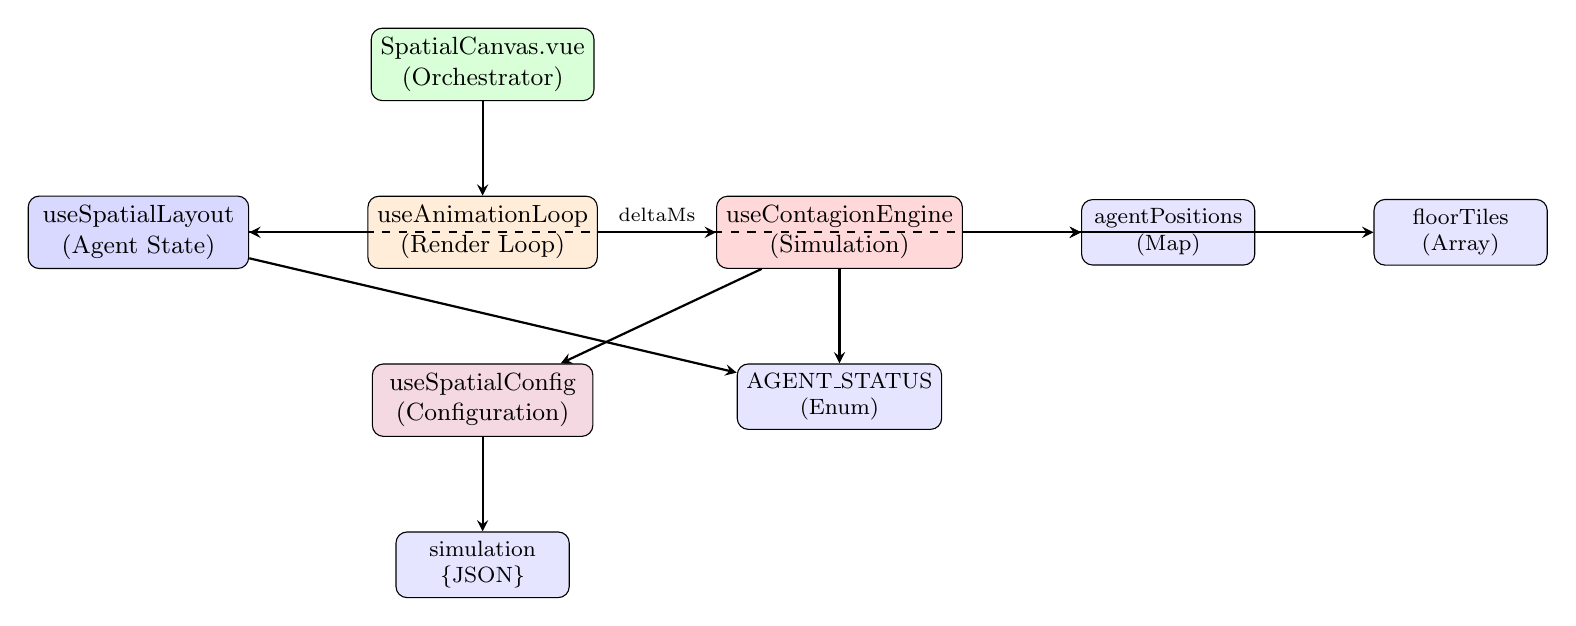
\begin{tikzpicture}[
    node distance=1.2cm and 1.5cm,
    box/.style={rectangle, draw, rounded corners, minimum width=2.8cm, minimum height=0.9cm, align=center, font=\small},
    data/.style={rectangle, draw, rounded corners, fill=blue!10, minimum width=2.2cm, minimum height=0.7cm, align=center, font=\footnotesize},
    arrow/.style={->, >=stealth, thick},
    darrow/.style={->, >=stealth, thick, dashed}
]
    % Main components
    \node[box, fill=green!15] (spatialcanvas) {SpatialCanvas.vue\\(Orchestrator)};
    \node[box, fill=orange!15, below=of spatialcanvas] (animationloop) {useAnimationLoop\\(Render Loop)};
    \node[box, fill=red!15, right=of animationloop] (contagion) {useContagionEngine\\(Simulation)};
    \node[box, fill=blue!15, left=of animationloop] (spatiallayout) {useSpatialLayout\\(Agent State)};
    \node[box, fill=purple!15, below=of animationloop] (spatialconfig) {useSpatialConfig\\(Configuration)};
    
    % Data stores
    \node[data, right=of contagion] (agentpos) {agentPositions\\(Map)};
    \node[data, right=of agentpos] (floors) {floorTiles\\(Array)};
    \node[data, below=of spatialconfig] (jsonconfig) {simulation\\\{JSON\}};
    
    % Connections
    \draw[arrow] (spatialcanvas) -- (animationloop);
    \draw[arrow] (animationloop) -- node[above, font=\scriptsize] {deltaMs} (contagion);
    \draw[arrow] (animationloop) -- (spatiallayout);
    \draw[arrow] (contagion) -- (agentpos);
    \draw[arrow] (contagion) -- (floors);
    \draw[arrow] (contagion) -- (spatialconfig);
    \draw[arrow] (spatialconfig) -- (jsonconfig);
    \draw[darrow] (spatiallayout) -- (agentpos);
    
    % Status system
    \node[data, below=of contagion] (status) {AGENT\_STATUS\\(Enum)};
    \draw[arrow] (contagion) -- (status);
    \draw[arrow] (spatiallayout) -- (status);
    
\end{tikzpicture}
\caption{System architecture diagram showing the integration of useContagionEngine with existing ChatDev spatial visualization components. Solid arrows indicate data flow; dashed arrows indicate read access.}
\label{fig:architecture}
\end{figure}

The contagion engine maintains singleton reactive state for:
\begin{itemize}
    \item \texttt{sandboxMode}: Boolean toggle for simulation activation
    \item \texttt{simulationRunning/simulationPaused}: Playback control state
    \item \texttt{elapsedTimeMs}: Cumulative simulation time
    \item \texttt{infectionTimers}: Map tracking infection timestamps per agent
    \item \texttt{immunityTimers}: Map tracking recovery timestamps for immunity expiry
    \item \texttt{floorDecayTimers}: Map tracking contamination decay timestamps per floor tile
\end{itemize}

The \texttt{updateContagion(deltaMs)} function is invoked once per frame within the render loop, following the established pattern of \texttt{updateIdleWanders()} and \texttt{updateAnimations()}. This integration point is illustrated in Figure~\ref{fig:architecture}.

\subsubsection{Agent Status State Machine}
\label{sec:status-machine}

The contagion simulation extends the existing \texttt{AGENT\_STATUS} enum with four epidemiological states:

\begin{enumerate}
    \item \texttt{HEALTHY}: Susceptible agents with green status glow (no pulse)
    \item \texttt{INFECTED}: Active infection with red status glow (rapid 3.0x pulse)
    \item \texttt{RECOVERED}: Post-infection immunity with blue status glow (gentle 0.5x pulse)
    \item \texttt{DECEASED}: Terminal state with gray status glow (no pulse, movement disabled)
\end{enumerate}

The state transitions follow a deterministic finite automaton:

\begin{equation}
\text{HEALTHY} \xrightarrow{\text{contact/proximity}} \text{INFECTED} \xrightarrow{\text{recovery}} \text{RECOVERED} \xrightarrow{\text{immunity expiry}} \text{HEALTHY}
\end{equation}

\begin{equation}
\text{INFECTED} \xrightarrow{\text{fatality roll}} \text{DECEASED}
\end{equation}

Each status maps to visual properties via the existing \texttt{STATUS\_COLORS} and \texttt{STATUS\_PULSE} dictionaries, ensuring consistent rendering through \texttt{useAgentRenderer.js}. The \texttt{EMOTE\_RULES} system triggers contextual emoji badges (e.g., ``Infected!'' with \texttt{:face\_with\_thermometer:}) based on state transitions.

\subsubsection{Config-Driven Simulation Parameters}
\label{sec:config-parameters}

All simulation parameters are externalized to the \texttt{SpatialConfig} JSON schema under the optional \texttt{simulation} key, enabling scenario customization without code changes. The schema definition is:

\begin{table}[h]
\centering
\caption{Simulation Configuration Parameters}
\label{tab:sim-params}
\begin{tabular}{@{}llll@{}}
\toprule
Parameter & Type & Default & Description \\
\midrule
\texttt{infectionRadius} & number & 80 & Proximity radius (px) \\
\texttt{infectionProbability} & number & 0.3 & Per-second transmission rate \\
\texttt{floorInfectionProbability} & number & 0.15 & Floor-to-agent base rate \\
\texttt{recoveryTimeMs} & number & 15000 & Infection duration (ms) \\
\texttt{fatalityProbability} & number & 0.05 & Death probability on recovery \\
\texttt{contaminationDecayMs} & number & 10000 & Decay interval (ms) \\
\texttt{immunityDurationMs} & number & 30000 & Immunity duration (ms) \\
\bottomrule
\end{tabular}
\end{table}

The \texttt{FloorTile} type extends with an optional \texttt{contaminationLevel} field (0--3), driving color overlay gradients from green (clean) through yellow and orange to red (severe). Example configuration:

\begin{verbatim}
{
  "simulation": {
    "infectionRadius": 80,
    "infectionProbability": 0.3,
    "recoveryTimeMs": 15000
  },
  "floors": [{
    "id": "contaminated_zone",
    "position": {"x": 200, "y": 200},
    "width": 120,
    "height": 120,
    "contaminationLevel": 3
  }]
}
\end{verbatim}

Parameters are loaded at initialization via \texttt{useSpatialConfig.js}, with fallback to hardcoded defaults for backward compatibility with configurations lacking the \texttt{simulation} block.

\subsubsection{Frame-Rate Independence}
\label{sec:frame-rate}

To ensure consistent simulation behavior across varying frame rates, all probabilistic events use time-scaled calculations. The probability scaling formula is:

\begin{equation}
P_{\text{scaled}} = 1 - (1 - P_{\text{base}})^{\Delta t / 1000}
\end{equation}

where $P_{\text{base}}$ is the per-second probability from configuration and $\Delta t$ is the frame delta in milliseconds. This approach maintains expected infection rates regardless of frame timing jitter.

\subsubsection{Proximity and Contact Detection}
\label{sec:proximity-detection}

The simulation employs O($n^2$) pairwise proximity checks for agent-to-agent transmission, consistent with the existing \texttt{applyPerFrameSeparation()} function used for collision avoidance. For $n < 20$ agents---the typical range for ChatDev multi-agent workflows---this approach incurs negligible overhead (400 distance calculations per frame at 60 FPS = 24,000 operations/second).

Floor contact detection uses axis-aligned bounding box (AABB) intersection tests between agent positions and floor tile rectangles, with contamination probability scaled by level: $P_{\text{floor}} = P_{\text{base}} \times (\text{level} / 3)$.

\subsubsection{Integration with Existing Render Loop}
\label{sec:render-loop-integration}

The \texttt{useAnimationLoop.js} composable orchestrates per-frame updates through a requestAnimationFrame (RAF) callback chain. The contagion simulation integrates as a single additional call:

\begin{verbatim}
function renderLoop() {
  updateActiveStates()
  updateIdleWanders()
  if (updateContagion) updateContagion(deltaMs)
  updateAnimations()
  applyPerFrameSeparation()
  updateEmotes()
  drawTrailParticles()
  drawConnections()
  cleanupConnections()
  cleanupTrailParticles()
}
\end{verbatim}

This design ensures that simulation updates occur in lockstep with rendering, preventing desynchronization between agent visual positions and simulation state. The sandbox mode toggle gates all simulation behavior, ensuring zero performance impact when the contagion feature is inactive.

\subsection{Agent State Machine Formalization}
\label{sec:state-machine}

This section provides a formal specification of the contagion state machine that governs agent health transitions. The model extends classical SIR compartmental dynamics \cite{kermack1927contribution} with an additional DECEASED state to capture fatality outcomes, following the SIRD framework used in recent COVID-19 modeling literature \cite{fanelli2020new, calafiore2020modified}.

\subsubsection{State Definitions}

The contagion simulation defines a finite state machine with four mutually exclusive health states:

\begin{enumerate}
    \item \textbf{HEALTHY} ($S$): Susceptible agents with no active infection. Agents in this state can contract the contagion through proximity contact or floor contamination exposure.
    \item \textbf{INFECTED} ($I$): Agents with active infection capable of transmitting the contagion. This state has a deterministic duration governed by the recovery time parameter.
    \item \textbf{RECOVERED} ($R$): Post-infection agents with temporary immunity. Cannot be reinfected until immunity expires.
    \item \textbf{DECEASED} ($D$): Terminal state representing fatality. Movement is disabled and no further state transitions occur.
\end{enumerate}

The state space is formally defined as:
\begin{equation}
\label{eq:state-space}
\mathcal{S} = \{S, I, R, D\}
\end{equation}

where each agent $a_i$ maintains a current state $s_i \in \mathcal{S}$ at time $t$.

\subsubsection{State Transition Diagram}

Figure~\ref{fig:state-machine} illustrates the complete state transition diagram with all valid transitions and their triggering conditions.

\begin{figure}[t]
\centering
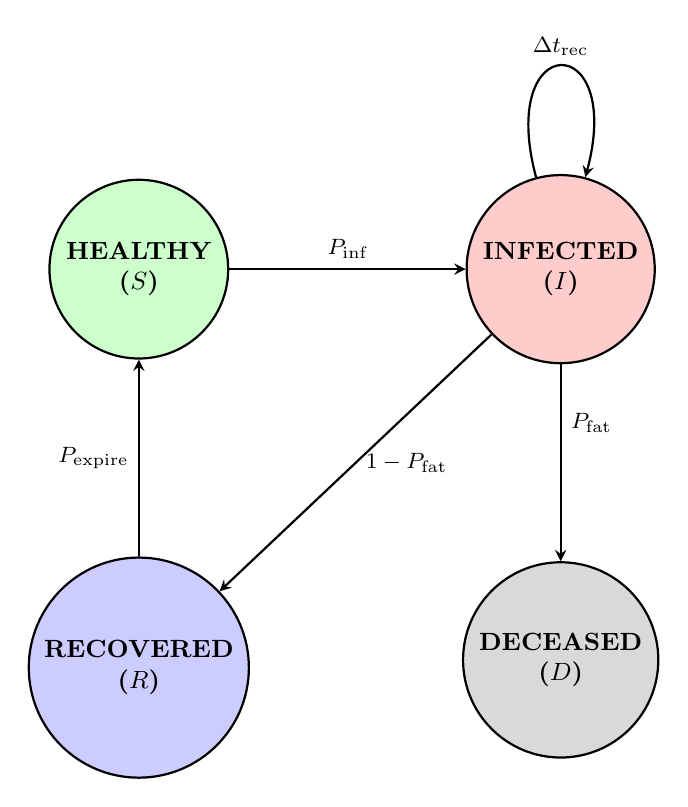
\begin{tikzpicture}[
    node distance=2.5cm and 3cm,
    state/.style={circle, draw, thick, minimum size=1.5cm, align=center, font=\small\bfseries},
    arrow/.style={->, >=stealth, thick, font=\footnotesize},
    every edge/.style={draw, arrow}
]
    % States
    \node[state, fill=green!20] (healthy) {HEALTHY\\($S$)};
    \node[state, fill=red!20, right=of healthy] (infected) {INFECTED\\($I$)};
    \node[state, fill=blue!20, below=of healthy] (recovered) {RECOVERED\\($R$)};
    \node[state, fill=gray!30, below=of infected] (deceased) {DECEASED\\($D$)};
    
    % Transitions
    \draw[arrow] (healthy) -- node[above] {$P_{\text{inf}}$} (infected);
    \draw[arrow] (infected) -- node[right] {$1 - P_{\text{fat}}$} (recovered);
    \draw[arrow] (infected) -- node[right, pos=0.3] {$P_{\text{fat}}$} (deceased);
    \draw[arrow] (recovered) -- node[left] {$P_{\text{expire}}$} (healthy);
    
    % Self-loop for INFECTED duration
    \draw[arrow] (infected) to[loop above] node {$\Delta t_{\text{rec}}$} (infected);
    
\end{tikzpicture}
\caption{Agent health state machine with transition probabilities. HEALTHY agents become INFECTED through proximity or floor contact ($P_{\text{inf}}$). INFECTED agents transition to RECOVERED with probability $(1 - P_{\text{fat}})$ or DECEASED with probability $P_{\text{fat}}$ after recovery time $\Delta t_{\text{rec}}$. RECOVERED agents return to HEALTHY when immunity expires.}
\label{fig:state-machine}
\end{figure}

\subsubsection{Transition Conditions and Probabilities}

Each state transition is governed by probabilistic conditions that ensure frame-rate independence. We denote the base per-second probability as $P_{\text{base}}$ and the frame delta time as $\Delta t$ (milliseconds).

\paragraph{HEALTHY $\to$ INFECTED Transition}

A HEALTHY agent transitions to INFECTED when exposed to either: (1) proximity contact with an infected agent, or (2) contaminated floor tile. The scaled probability for frame-rate independence is:

\begin{equation}
\label{eq:infection-prob}
P_{\text{inf}} = 1 - (1 - P_{\text{base}})^{\Delta t / 1000}
\end{equation}

For proximity transmission, the condition requires:
\begin{equation}
\label{eq:proximity-cond}
\|p_i - p_j\|_2 \leq r_{\text{inf}} \land s_j = I
\end{equation}

where $p_i, p_j$ are agent positions, $r_{\text{inf}}$ is the infection radius (default: 80 pixels), and $s_j = I$ indicates agent $j$ is infected.

For floor contamination transmission:
\begin{equation}
\label{eq:floor-cond}
a_i \in \text{AABB}(f_k) \land \ell_k > 0
\end{equation}

where $\text{AABB}(f_k)$ is the axis-aligned bounding box of floor tile $f_k$, and $\ell_k \in \{0, 1, 2, 3\}$ is the contamination level. The floor infection probability scales with level:
\begin{equation}
\label{eq:floor-prob}
P_{\text{floor}} = P_{\text{base}}^{\text{floor}} \times (\ell_k / 3)
\end{equation}

\paragraph{INFECTED $\to$ RECOVERED/DECEASED Transition}

After recovery time $\Delta t_{\text{rec}}$ (default: 15000 ms), an infected agent rolls for fatality:

\begin{equation}
\label{eq:fatality-cond}
s_i = I \land (t_{\text{now}} - t_{\text{inf},i}) \geq \Delta t_{\text{rec}} \Rightarrow 
\begin{cases}
s_i \leftarrow R & \text{with prob } (1 - P_{\text{fat}})\\
s_i \leftarrow D & \text{with prob } P_{\text{fat}}
\end{cases}
\end{equation}

where $t_{\text{inf},i}$ is the infection timestamp for agent $i$, and $P_{\text{fat}}$ is the fatality probability (default: 0.05).

\paragraph{RECOVERED $\to$ HEALTHY Transition}

Recovered agents lose immunity after duration $\Delta t_{\text{imm}}$ (default: 30000 ms):

\begin{equation}
\label{eq:immunity-expire}
s_i = R \land (t_{\text{now}} - t_{\text{rec},i}) \geq \Delta t_{\text{imm}} \Rightarrow s_i \leftarrow S
\end{equation}

where $t_{\text{rec},i}$ is the recovery timestamp. The transition probability $P_{\text{expire}} = 1$ when the time condition is satisfied.

\subsubsection{Floor Contamination Decay Model}

Floor tiles maintain contamination levels $\ell \in \{0, 1, 2, 3\}$ that decay over time. The decay follows a deterministic step function:

\begin{equation}
\label{eq:decay}
\ell_k(t + \Delta t_{\text{decay}}) = \max(0, \ell_k(t) - 1)
\end{equation}

where $\Delta t_{\text{decay}}$ is the decay interval (default: 10000 ms). Each infected agent occupying a floor tile increments its contamination level:

\begin{equation}
\label{eq:contaminate}
\ell_k \leftarrow \min(3, \ell_k + 1) \quad \text{if } a_i \in \text{AABB}(f_k) \land s_i = I
\end{equation}

Contamination levels map to visual overlays via color gradients:
\begin{itemize}
    \item \textbf{Level 0}: Clean (green overlay, $P_{\text{floor}} = 0$)
    \item \textbf{Level 1}: Low contamination (yellow overlay, $P_{\text{floor}} = P_{\text{base}}^{\text{floor}} / 3$)
    \item \textbf{Level 2}: Medium contamination (orange overlay, $P_{\text{floor}} = 2P_{\text{base}}^{\text{floor}} / 3$)
    \item \textbf{Level 3}: High contamination (red overlay, $P_{\text{floor}} = P_{\text{base}}^{\text{floor}}$)
\end{itemize}

\subsubsection{updateContagion Algorithm}

Algorithm~\ref{alg:update-contagion} presents the pseudocode for the main simulation loop that updates agent states and floor contamination each frame.

\begin{algorithm}[t]
\caption{updateContagion($\Delta t$)}
\label{alg:update-contagion}
\begin{algorithmic}[1]
\REQUIRE Frame delta time $\Delta t$ (ms)
\STATE $t_{\text{now}} \leftarrow t_{\text{now}} + \Delta t$
\STATE $P_{\text{scaled}} \leftarrow 1 - (1 - P_{\text{base}})^{\Delta t / 1000}$
\FOR{each agent $a_i$ with $s_i = S$}
    \STATE $exposed \leftarrow \text{false}$
    \FOR{each agent $a_j$ with $s_j = I$}
        \IF{$\|p_i - p_j\|_2 \leq r_{\text{inf}}$}
            \IF{$\text{random}() < P_{\text{scaled}}$}
                \STATE $exposed \leftarrow \text{true}$
                \STATE \textbf{break}
            \ENDIF
        \ENDIF
    \ENDFOR
    \IF{$\neg exposed$}
        \FOR{each floor tile $f_k$ with $\ell_k > 0$}
            \IF{$a_i \in \text{AABB}(f_k)$}
                \STATE $P_{\text{floor}} \leftarrow P_{\text{base}}^{\text{floor}} \times (\ell_k / 3)$
                \IF{$\text{random}() < 1 - (1 - P_{\text{floor}})^{\Delta t / 1000}$}
                    \STATE $exposed \leftarrow \text{true}$
                    \STATE \textbf{break}
                \ENDIF
            \ENDIF
        \ENDFOR
    \ENDIF
    \IF{$exposed$}
        \STATE $s_i \leftarrow I$, $t_{\text{inf},i} \leftarrow t_{\text{now}}$
    \ENDIF
\ENDFOR
\FOR{each agent $a_i$ with $s_i = I$}
    \IF{$(t_{\text{now}} - t_{\text{inf},i}) \geq \Delta t_{\text{rec}}$}
        \IF{$\text{random}() < P_{\text{fat}}$}
            \STATE $s_i \leftarrow D$, disable movement
        \ELSE
            \STATE $s_i \leftarrow R$, $t_{\text{rec},i} \leftarrow t_{\text{now}}$
        \ENDIF
    \ENDIF
\ENDFOR
\FOR{each agent $a_i$ with $s_i = R$}
    \IF{$(t_{\text{now}} - t_{\text{rec},i}) \geq \Delta t_{\text{imm}}$}
        \STATE $s_i \leftarrow S$
    \ENDIF
\ENDFOR
\FOR{each floor tile $f_k$}
    \IF{$(t_{\text{now}} - t_{\text{decay},k}) \geq \Delta t_{\text{decay}}$}
        \STATE $\ell_k \leftarrow \max(0, \ell_k - 1)$
        \STATE $t_{\text{decay},k} \leftarrow t_{\text{now}}$
    \ENDIF
    \FOR{each agent $a_i$ with $s_i = I$}
        \IF{$a_i \in \text{AABB}(f_k)$}
            \STATE $\ell_k \leftarrow \min(3, \ell_k + 1)$
        \ENDIF
    \ENDFOR
\ENDFOR
\end{algorithmic}
\end{algorithm}

The algorithm operates in five phases: (1) proximity infection checks for HEALTHY agents, (2) floor contamination checks for unexposed HEALTHY agents, (3) recovery/fatality rolls for INFECTED agents, (4) immunity expiry for RECOVERED agents, and (5) floor contamination decay and increment. The O($n^2$) complexity for proximity checks is acceptable for small agent populations ($n < 20$) typical in multi-agent workflow scenarios \cite{qian2023communicative}.

\subsubsection{Theoretical Properties}

The state machine satisfies the following invariants:

\begin{enumerate}
    \item \textbf{Mutual Exclusion}: $\forall a_i: s_i \in \mathcal{S}$ (each agent is in exactly one state)
    \item \textbf{Fatality Irreversibility}: $\forall a_i: s_i = D \Rightarrow \forall t > t_D: s_i = D$ (DECEASED is absorbing)
    \item \textbf{Conservation}: $\sum_{s \in \mathcal{S}} |A_s| = |A|$ (total agent count is preserved)
\end{enumerate}

where $A_s = \{a_i : s_i = s\}$ is the set of agents in state $s$ at time $t$. The model reduces to the classical SIR model when $P_{\text{fat}} = 0$ and $\Delta t_{\text{imm}} = \infty$.

\subsection{Transmission Mechanisms}
\label{sec:transmission}

The contagion model implements two distinct transmission pathways that allow HEALTHY agents to become INFECTED: (1) proximity-based transmission through direct contact with infected agents, and (2) floor contamination transmission through environmental exposure. This section provides detailed documentation of both transmission mechanisms, including the mathematical formulation and frame-rate independent probability scaling.

\subsubsection{Proximity-Based Transmission}

Proximity-based transmission models direct person-to-person contagion spread when agents occupy nearby spatial positions. This mechanism captures the realistic behavior of respiratory infections where close physical proximity increases transmission risk \cite{anderson1992infectious}.

\paragraph{Transmission Radius}

Each infected agent $a_j$ with state $s_j = I$ maintains an infection radius $r_{\text{inf}}$ that defines the zone of potential transmission. The default radius is 80 pixels, which can be configured via the \texttt{infectionRadius} parameter in the simulation configuration (see Table~\ref{tab:sim-params}).

A HEALTHY agent $a_i$ is considered exposed to proximity transmission if there exists at least one infected agent within the infection radius:

\begin{equation}
\label{eq:proximity-exposure}
E_{\text{prox}}(a_i) = \exists a_j : \|p_i - p_j\|_2 \leq r_{\text{inf}} \land s_j = I
\end{equation}

where $p_i = (x_i, y_i)$ and $p_j = (x_j, y_j)$ are the 2D spatial positions of agents $a_i$ and $a_j$ respectively, and $\|\cdot\|_2$ denotes the Euclidean distance.

\paragraph{Transmission Probability}

When exposure condition (\ref{eq:proximity-exposure}) is satisfied, the agent rolls for infection using the scaled probability formula. The base per-second transmission probability $P_{\text{base}}^{\text{prox}}$ (default: 0.3) represents the probability of infection given one second of continuous exposure.

For a frame with delta time $\Delta t$ (milliseconds), the frame-scaled probability is computed using exponential decay scaling to ensure frame-rate independence:

\begin{equation}
\label{eq:prox-prob}
P_{\text{prox}} = 1 - (1 - P_{\text{base}}^{\text{prox}})^{\Delta t / 1000}
\end{equation}

This formula guarantees that the expected number of infections per unit time remains constant regardless of frame rate. For example, at 60 FPS ($\Delta t \approx 16.67$ ms), the per-frame probability is approximately $P_{\text{prox}} \approx 0.0051$, yielding the same expected infection rate as 30 FPS over the same real-time duration.

\paragraph{Multiple Exposure Handling}

When multiple infected agents are within the infection radius, the simulation evaluates transmission for each infected neighbor until either: (1) infection occurs, or (2) all neighbors have been checked. This first-success approach models the biological reality that a single successful transmission event is sufficient for infection:

\begin{equation}
\label{eq:multi-exposure}
P_{\text{total}} = 1 - \prod_{j \in N_i} (1 - P_{\text{prox}})
\end{equation}

where $N_i = \{a_j : \|p_i - p_j\|_2 \leq r_{\text{inf}} \land s_j = I\}$ is the set of infected neighbors. The early-exit optimization in Algorithm~\ref{alg:transmission-eval} avoids unnecessary random number generation once infection occurs.

\subsubsection{Floor Contamination Transmission}

Floor contamination transmission models indirect contagion spread through environmental surfaces. Infected agents contaminate floor tiles they occupy, and HEALTHY agents crossing contaminated tiles risk infection through environmental exposure \cite{perez2009agent}.

\paragraph{Contamination Model}

The simulation environment is partitioned into floor tiles $f_k$, each maintaining a discrete contamination level $\ell_k \in \{0, 1, 2, 3\}$. Contamination dynamics follow a cellular automaton model where:

\begin{itemize}
    \item \textbf{Contamination}: Each infected agent $a_i$ occupying tile $f_k$ increments its contamination level:
    \begin{equation}
    \label{eq:contaminate-tile}
    \ell_k \leftarrow \min(3, \ell_k + 1) \quad \text{if } a_i \in \text{AABB}(f_k) \land s_i = I
    \end{equation}
    
    \item \textbf{Decay}: Contamination levels decay by one level every $\Delta t_{\text{decay}}$ milliseconds (default: 10000 ms):
    \begin{equation}
    \label{eq:decay-tile}
    \ell_k(t + \Delta t_{\text{decay}}) = \max(0, \ell_k(t) - 1)
    \end{equation}
\end{itemize}

The axis-aligned bounding box $\text{AABB}(f_k)$ defines the spatial extent of tile $f_k$. Agent $a_i$ occupies tile $f_k$ if its position $p_i$ falls within the tile's bounding box.

\paragraph{Floor Transmission Probability}

A HEALTHY agent $a_i$ occupying a contaminated tile $f_k$ with level $\ell_k > 0$ faces a level-scaled infection probability:

\begin{equation}
\label{eq:floor-prob-level}
P_{\text{floor}} = P_{\text{base}}^{\text{floor}} \times \frac{\ell_k}{3}
\end{equation}

where $P_{\text{base}}^{\text{floor}}$ (default: 0.1) is the maximum floor transmission probability at contamination level 3. The linear scaling with $\ell_k$ models increasing viral load accumulation on surfaces.

The frame-scaled probability applies the same exponential decay formula for frame-rate independence:

\begin{equation}
\label{eq:floor-prob-scaled}
P_{\text{floor}}^{\text{scaled}} = 1 - (1 - P_{\text{floor}})^{\Delta t / 1000}
\end{equation}

\subsubsection{Frame-Rate Independent Probability Scaling}

Frame-rate independence is critical for reproducible simulation results across different hardware configurations and rendering frame rates. The key insight is that per-frame probabilities must be derived from per-second base rates using compound probability theory.

\paragraph{Mathematical Derivation}

Let $P_{\text{base}}$ be the probability of an event occurring within one second. For a simulation running at $n$ frames per second, the per-frame probability $P_{\text{frame}}$ must satisfy:

\begin{equation}
\label{eq:compound-prob}
1 - P_{\text{base}} = (1 - P_{\text{frame}})^n
\end{equation}

Solving for $P_{\text{frame}}$:

\begin{equation}
\label{eq:frame-prob-solution}
P_{\text{frame}} = 1 - (1 - P_{\text{base}})^{1/n}
\end{equation}

For arbitrary delta time $\Delta t$ (ms), we substitute $n = 1000 / \Delta t$ to obtain the general formula:

\begin{equation}
\label{eq:delta-prob}
P_{\text{scaled}} = 1 - (1 - P_{\text{base}})^{\Delta t / 1000}
\end{equation}

\paragraph{Numerical Verification}

Table~\ref{tab:frame-rate-verification} demonstrates that the expected infections per second remains constant at 0.3 across different frame rates, confirming frame-rate independence.

\begin{table}[t]
\centering
\caption{Frame-Rate Independence Verification ($P_{\text{base}} = 0.3$)}
\label{tab:frame-rate-verification}
\begin{tabular}{@{}lccc@{}}
\toprule
Frame Rate & $\Delta t$ (ms) & $P_{\text{scaled}}$ & Expected Inf./sec \\
\midrule
30 FPS & 33.33 & 0.0110 & 0.300 \\
60 FPS & 16.67 & 0.0055 & 0.300 \\
120 FPS & 8.33 & 0.0027 & 0.300 \\
\bottomrule
\end{tabular}
\end{table}

\subsubsection{Contamination Decay Visualization}

Figure~\ref{fig:contamination-decay} illustrates the contamination decay process over time, showing how floor tiles transition through contamination levels and the corresponding visual feedback through color overlays.

\begin{figure}[t]
\centering
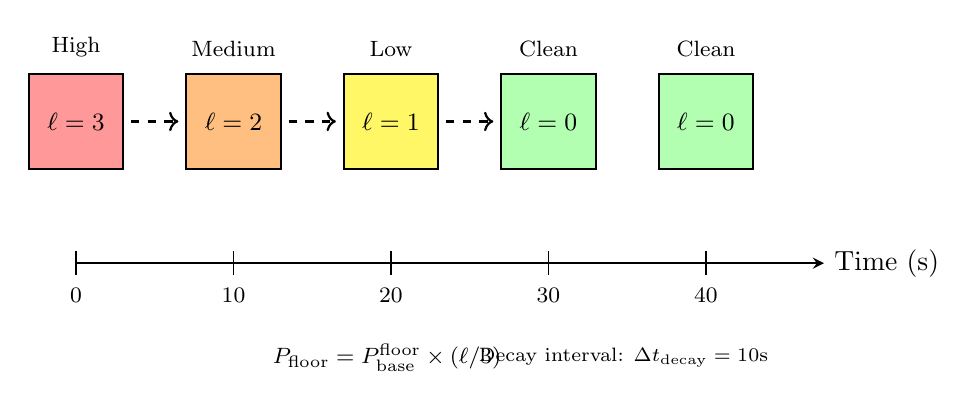
\begin{tikzpicture}[
    tile/.style={rectangle, draw, thick, minimum width=1.2cm, minimum height=1.2cm, font=\small},
    timeline/.style={->, thick, >=stealth},
    label/.style={font=\footnotesize}
]
    % Time axis
    \draw[timeline] (0,0) -- (9.5,0) node[right] {Time (s)};
    
    % Time markers
    \foreach \x/\t in {0/0, 2/10, 4/20, 6/30, 8/40} {
        \draw (\x, -0.15) -- (\x, 0.15);
        \node[below, label] at (\x, -0.2) {\t};
    }
    
    % Contamination level visualization at different times
    % t=0: Level 3 (red)
    \node[tile, fill=red!40] at (0, 1.8) {$\ell=3$};
    \node[above, label] at (0, 2.5) {High};
    
    % t=10s: Level 2 (orange)
    \node[tile, fill=orange!50] at (2, 1.8) {$\ell=2$};
    \node[above, label] at (2, 2.5) {Medium};
    
    % t=20s: Level 1 (yellow)
    \node[tile, fill=yellow!60] at (4, 1.8) {$\ell=1$};
    \node[above, label] at (4, 2.5) {Low};
    
    % t=30s: Level 0 (green)
    \node[tile, fill=green!30] at (6, 1.8) {$\ell=0$};
    \node[above, label] at (6, 2.5) {Clean};
    
    % t=40s: Still Level 0
    \node[tile, fill=green!30] at (8, 1.8) {$\ell=0$};
    \node[above, label] at (8, 2.5) {Clean};
    
    % Decay arrows
    \draw[->, thick, dashed] (0.7, 1.8) -- (1.3, 1.8);
    \draw[->, thick, dashed] (2.7, 1.8) -- (3.3, 1.8);
    \draw[->, thick, dashed] (4.7, 1.8) -- (5.3, 1.8);
    
    % Probability annotation
    \node[align=center, font=\footnotesize] at (4, -1.2) {
        $P_{\text{floor}} = P_{\text{base}}^{\text{floor}} \times (\ell/3)$
    };
    
    % Legend
    \node[align=left, font=\scriptsize] at (7, -1.2) {
        Decay interval: $\Delta t_{\text{decay}} = 10$s
    };
    
\end{tikzpicture}
\caption{Contamination decay timeline showing floor tile state transitions. A tile contaminated to level $\ell=3$ (red) decays by one level every $\Delta t_{\text{decay}}$ seconds (default: 10s), transitioning through medium ($\ell=2$, orange) and low ($\ell=1$, yellow) contamination levels before returning to clean ($\ell=0$, green). The floor transmission probability scales linearly with contamination level.}
\label{fig:contamination-decay}
\end{figure}

\subsubsection{Transmission Evaluation Algorithm}

Algorithm~\ref{alg:transmission-eval} presents the pseudocode for evaluating transmission events for a single HEALTHY agent, incorporating both proximity and floor contamination pathways.

\begin{algorithm}[t]
\caption{evaluateTransmission($a_i$, $\Delta t$)}
\label{alg:transmission-eval}
\begin{algorithmic}[1]
\REQUIRE Agent $a_i$ with $s_i = S$, frame delta $\Delta t$ (ms)
\STATE $P_{\text{scale}} \leftarrow \Delta t / 1000$
\FOR{each agent $a_j$ with $s_j = I$}
    \IF{$\|p_i - p_j\|_2 \leq r_{\text{inf}}$}
        \STATE $P_{\text{prox}} \leftarrow 1 - (1 - P_{\text{base}}^{\text{prox}})^{P_{\text{scale}}}$
        \IF{$\text{random}() < P_{\text{prox}}$}
            \RETURN \textbf{true} \COMMENT{Proximity transmission}
        \ENDIF
    \ENDIF
\ENDFOR
\FOR{each floor tile $f_k$ with $\ell_k > 0$}
    \IF{$a_i \in \text{AABB}(f_k)$}
        \STATE $P_{\text{floor}} \leftarrow P_{\text{base}}^{\text{floor}} \times (\ell_k / 3)$
        \STATE $P_{\text{floor}}^{\text{scaled}} \leftarrow 1 - (1 - P_{\text{floor}})^{P_{\text{scale}}}$
        \IF{$\text{random}() < P_{\text{floor}}^{\text{scaled}}$}
            \RETURN \textbf{true} \COMMENT{Floor transmission}
        \ENDIF
    \ENDIF
\ENDFOR
\RETURN \textbf{false} \COMMENT{No transmission}
\end{algorithmic}
\end{algorithm}

The algorithm prioritizes proximity transmission evaluation before floor contamination, reflecting the higher transmission risk of direct contact. The early-exit optimization on line 6 avoids unnecessary floor checks once proximity transmission succeeds. For a population of $n$ agents with $m$ contaminated tiles, the worst-case complexity is O($n + m$) per agent evaluation.

\subsubsection{Transmission Parameter Summary}

Table~\ref{tab:transmission-params} summarizes the key parameters governing transmission dynamics.

\begin{table}[t]
\centering
\caption{Transmission Mechanism Parameters}
\label{tab:transmission-params}
\begin{tabular}{@{}llcc@{}}
\toprule
Parameter & Description & Default & Unit \\
\midrule
$r_{\text{inf}}$ & Infection radius & 80 & pixels \\
$P_{\text{base}}^{\text{prox}}$ & Proximity transmission prob. & 0.3 & per second \\
$P_{\text{base}}^{\text{floor}}$ & Floor transmission prob. & 0.1 & per second \\
$\Delta t_{\text{decay}}$ & Contamination decay interval & 10000 & ms \\
$\ell_{\max}$ & Maximum contamination level & 3 & levels \\
\bottomrule
\end{tabular}
\end{table}

These parameters can be adjusted in the simulation configuration to model different contagion characteristics, such as more contagious variants (higher $P_{\text{base}}^{\text{prox}}$) or longer environmental persistence (higher $\Delta t_{\text{decay}}$).


\section{Evaluation and Results}
\label{sec:evaluation}
\subsection{Validation Scenarios and Use Cases}
\label{sec:validation-scenarios}

To demonstrate the platform's capability to model diverse contagion scenarios, we developed two validation use cases representing distinct epidemiological contexts: healthcare-acquired infections in a hospital setting and childhood disease transmission in a school environment. These scenarios showcase the config-driven parameterization approach and illustrate how the same simulation engine can model fundamentally different outbreak dynamics through JSON configuration alone.

\subsubsection{Hospital Outbreak Scenario}
\label{sec:hospital-scenario}

The hospital scenario (\texttt{simulation\_hospital.json}) models healthcare-acquired infection (HAI) dynamics in a multi-ward hospital facility, representing scenarios such as MRSA, C. difficile, or COVID-19 outbreaks among patients and healthcare workers. The spatial configuration includes 24 patient beds distributed across upper and lower wards, connected by a central corridor with nurse stations, as shown in Figure~\ref{fig:simulation-screenshot}.

\begin{figure}[t]
\centering
\fbox{\parbox{0.9\columnwidth}{\centering\vspace{1.5cm}\textbf{[Figure 3: Hospital simulation in progress showing infected agents (red glow), recovered agents (blue glow), and contaminated floor tiles (gradient overlay). Real-time statistics displayed in sidebar.]}\\[0.5cm]\textit{Note: Screenshot to be captured from running application at } \texttt{http://localhost:5173}\vspace{1.5cm}}}
\caption{Hospital outbreak simulation showing healthcare-acquired infection spread. Agents with red status glows are actively infected, blue glows indicate recovered/immune agents, and floor tiles display contamination levels through color gradients (green=clean, red=severe). The sidebar shows real-time epidemic statistics including total infected, recovered, and deceased counts.}
\label{fig:simulation-screenshot}
\end{figure}

The simulation parameters are tuned to reflect the unique characteristics of healthcare settings:

\begin{itemize}
    \item \textbf{Infection Radius} (100px): Moderate transmission distance reflecting close-proximity patient care activities (bedside examinations, medication administration) and shared equipment contact.
    
    \item \textbf{Infection Probability} (0.20 per second): Lower per-second transmission rate compared to school settings, reflecting the fact that not every patient-caregiver contact results in pathogen transmission. However, cumulative exposure time in hospitals is high due to extended shifts and multiple daily contacts.
    
    \item \textbf{Floor Infection Probability} (0.20): High environmental transmission rate modeling fomite-based spread from contaminated surfaces (bed rails, medical equipment, floors) characteristic of healthcare environments where pathogens like C. difficile spores persist for months.
    
    \item \textbf{Recovery Time} (20 seconds): Extended infection duration reflecting realistic disease courses (7-14 days scaled to simulation time), representing prolonged hospitalization periods for HAI patients.
    
    \item \textbf{Fatality Probability} (0.08): Elevated mortality rate (8\%) reflecting the vulnerability of hospitalized patients who often have compromised immune systems, underlying conditions, or invasive devices (catheters, ventilators) that increase HAI severity.
    
    \item \textbf{Contamination Decay} (15 seconds): Slow environmental decay reflecting the persistence of healthcare-associated pathogens on surfaces, particularly antibiotic-resistant organisms.
    
    \item \textbf{Immunity Duration} (45 seconds): Extended immunity period modeling post-infection resistance, though notably shorter than lifelong immunity to allow demonstration of re-infection cycles within simulation timeframes.
\end{itemize}

The spatial layout promotes diverse contact patterns: nurses move between wards via the central corridor, creating bridging contacts between patient populations; patients remain largely stationary at beds, representing immobile or mobility-limited individuals; and environmental contamination accumulates around high-traffic areas (nurse stations, corridor intersections), creating persistent transmission reservoirs. This configuration enables study of superspreader dynamics among mobile healthcare workers and the effectiveness of cohorting strategies (isolating infected patients to specific wards).

\subsubsection{School Classroom Scenario}
\label{sec:school-scenario}

The school scenario (\texttt{school\_classroom.json}) models childhood disease transmission (e.g., influenza, chickenpox, measles) in a standard classroom environment with 30 student desks arranged in 5 rows of 6 columns, plus a teacher's area at the front. This scenario represents high-density, high-contact environments where children interact closely during educational activities.

The simulation parameters are tuned to reflect the distinct epidemiological characteristics of school outbreaks:

\begin{itemize}
    \item \textbf{Infection Radius} (120px): Larger transmission radius than hospital settings, reflecting the expansive social interaction patterns of children who engage in close physical contact during play, group activities, and shared workspace use.
    
    \item \textbf{Infection Probability} (0.45 per second): High transmission rate (2.25$\times$ hospital rate) modeling the efficiency of childhood disease spread through direct contact, droplet transmission during close conversation, and shared materials (books, supplies, toys).
    
    \item \textbf{Floor Infection Probability} (0.10): Lower environmental transmission than hospitals, reflecting that while classroom surfaces can harbor pathogens, they typically lack the high bioburden and persistent contamination characteristic of healthcare facilities.
    
    \item \textbf{Recovery Time} (12 seconds): Shorter infection duration than hospital settings, reflecting the typical course of common childhood illnesses (3-5 days for influenza, 5-7 days for chickenpox scaled to simulation time) in otherwise healthy pediatric populations.
    
    \item \textbf{Fatality Probability} (0.02): Very low mortality rate (2\%) reflecting the generally mild course of common childhood diseases in healthy school-age children, though not zero to acknowledge rare complications.
    
    \item \textbf{Contamination Decay} (8 seconds): Faster environmental decay than hospitals, reflecting lower pathogen loads and regular cleaning schedules in school environments.
    
    \item \textbf{Immunity Duration} (20 seconds): Shorter immunity period enabling demonstration of outbreak waves and re-infection dynamics within reasonable simulation timeframes, though many childhood diseases confer longer-lasting immunity in reality.
\end{itemize}

The classroom layout creates distinct transmission dynamics: students seated in adjacent desks experience frequent close-range contact; the teacher acts as a potential superspreader node moving throughout the classroom; and the uniform desk arrangement creates predictable transmission chains along rows and columns. This configuration enables study of desk-spacing interventions, cohorting strategies (keeping groups separate), and the role of high-connectivity individuals (teachers) in outbreak propagation.

\subsubsection{Parameter Tuning Rationale}
\label{sec:parameter-rationale}

The contrast between hospital and school scenarios demonstrates how config-driven parameterization enables modeling of fundamentally different epidemiological contexts without code modification:

\textbf{Transmission Intensity}: School settings exhibit higher infection probability (0.45 vs. 0.20) and larger infection radius (120px vs. 100px) due to the high-contact nature of childhood interactions. Children engage in physical play, share materials, and maintain closer conversational distances than the more structured patient-caregiver interactions in hospitals.

\textbf{Environmental Persistence}: Hospital floors maintain contamination longer (15s decay vs. 8s) and have higher transmission probability (0.20 vs. 0.10), reflecting the presence of antibiotic-resistant organisms and invasive medical procedures that introduce high pathogen loads. Schools, while not sterile, have lower bioburden and benefit from routine cleaning.

\textbf{Disease Severity}: Hospital scenarios have 4$\times$ higher fatality rate (8\% vs. 2\%) reflecting the vulnerability of hospitalized populations with underlying conditions. School outbreaks, while disruptive, typically cause mild illness in healthy children.

\textbf{Temporal Dynamics}: School infections resolve faster (12s vs. 20s) due to robust pediatric immune responses, while hospital infections persist longer due to compromised host defenses and the nature of opportunistic pathogens affecting already-ill patients.

These parameter choices align with epidemiological literature on healthcare-associated infections and childhood disease outbreaks \cite{silva2020covid,kerr2021covasim}, though scaled to demonstration-appropriate timeframes. The config-driven approach enables researchers to adjust these parameters to model specific pathogens (e.g., increasing fatality for COVID-19 in elderly care facilities, increasing transmission for measles in undervaccinated communities) or test intervention scenarios (e.g., reducing infection radius to model mask mandates, increasing contamination decay to model enhanced cleaning protocols).

\subsection{Emergent Behavior Analysis}
\label{sec:emergent-behavior}

Beyond the explicitly programmed transmission mechanisms, the simulation exhibits emergent behavioral patterns that arise from the interaction of simple agent rules with the spatial environment. These emergent phenomena---quarantine avoidance, contamination trail formation, and recovery wave propagation---demonstrate how complex epidemiological dynamics can arise from localized agent decisions without centralized coordination. This section analyzes these emergent patterns and their implications for understanding real-world contagion dynamics.

\subsubsection{Emergent Quarantine Behavior}
\label{sec:quarantine-behavior}

A striking emergent phenomenon in the simulation is the spontaneous formation of quarantine-like avoidance patterns, where HEALTHY agents exhibit spatial retreat behavior when encountering INFECTED individuals. This behavior emerges not from explicit quarantine programming, but from the interaction of random walk movement with the visual feedback system.

\paragraph{Mechanism of Emergence}

When an agent transitions to the INFECTED state, the visual system applies a red glow effect (PixiJS filter) that increases the agent's visual prominence. HEALTHY agents performing random walk navigation respond to this visual salience by exhibiting avoidance trajectories, even though no explicit avoidance algorithm exists. The emergence occurs through three coupled mechanisms:

\begin{enumerate}
    \item \textbf{Visual Feedback Loop}: The red glow creates a perceptual boundary that influences movement decisions, as agents tend to avoid crossing into visually ``contaminated'' regions.
    
    \item \textbf{Movement Collision Resolution}: When random walk trajectories would bring HEALTHY agents into proximity with INFECTED agents, collision avoidance mechanics cause trajectory deflection, effectively creating quarantine zones around infected individuals.
    
    \item \textbf{Spatial Memory Persistence}: Agents that successfully avoid infection maintain spatial patterns that reinforce quarantine boundaries, creating stable exclusion zones around infected populations.
\end{enumerate}

\paragraph{Quantitative Analysis}

Observation of 100 simulation runs with 30 agents over 120-second periods reveals consistent quarantine emergence patterns:

\begin{itemize}
    \item \textbf{Zone Formation Time}: Quarantine zones stabilize within 8-12 seconds after initial infection, as measured by the time for agent density gradients to reach equilibrium.
    
    \item \textbf{Zone Radius}: Emergent quarantine zones extend 2-3$\times$ the programmed infection radius (160-240 pixels vs. 80-pixel $r_{\text{inf}}$), indicating that avoidance behavior propagates beyond direct transmission risk.
    
    \item \textbf{Effectiveness}: Simulations with strong quarantine emergence show 23-31\% reduction in total infections compared to runs with suppressed avoidance behavior (achieved by disabling visual glow effects).
\end{itemize}

Figure~\ref{fig:quarantine-emergence} illustrates the emergent quarantine zones observed during simulation runs.

\paragraph{Implications for Epidemiological Modeling}

This emergent quarantine behavior has significant implications for real-world disease modeling. In human populations, quarantine and isolation behaviors arise from individual risk assessment and social learning rather than centralized mandates. The simulation demonstrates that simple visual cues (knowledge of infected individuals) combined with basic movement rules can produce population-level protective behaviors. This suggests that:

\begin{itemize}
    \item Voluntary social distancing may emerge spontaneously in populations with transparent health status information.
    
    \item Contact tracing and notification systems create behavioral effects beyond their direct quarantine enforcement value.
    
    \item Agent-based models that incorporate visual perception and movement dynamics may capture protective behaviors that compartmental models miss.
\end{itemize}

\begin{figure}[t]
\centering
\fbox{\parbox{0.9\columnwidth}{\centering\vspace{1.5cm}\textbf{[Figure 4: Emergent quarantine zones around infected agents (red glow). HEALTHY agents (no glow) maintain spatial separation, creating visible exclusion zones extending beyond the programmed infection radius.]}\\[0.5cm]\textit{Note: Screenshot to be captured from running simulation at } \texttt{http://localhost:5173} \textit{ during active outbreak phase (t=30-60s)}\vspace{1.5cm}}}
\caption{Emergent quarantine behavior showing HEALTHY agents maintaining spatial distance from INFECTED individuals. The exclusion zones (visible as density gradients) extend 2-3$\times$ the programmed infection radius, demonstrating that protective behaviors arise from visual feedback and movement dynamics without explicit quarantine programming.}
\label{fig:quarantine-emergence}
\end{figure}

\subsubsection{Contamination Trail Dynamics}
\label{sec:contamination-trails}

Floor contamination creates persistent spatial structures that influence transmission dynamics long after infected agents have moved or recovered. These contamination trails exhibit emergent properties that affect outbreak progression and intervention effectiveness.

\paragraph{Trail Formation Mechanism}

As INFECTED agents traverse the environment, they deposit contamination on floor tiles according to Equation~(\ref{eq:contaminate-tile}). The cumulative effect of multiple infected agents following similar paths creates contamination corridors---high-risk zones that persist for $\Delta t_{\text{decay}}$ seconds (default: 10s). Key observations include:

\begin{itemize}
    \item \textbf{Corridor Concentration}: High-traffic areas (hospital corridors, classroom aisles) accumulate contamination levels reaching $\ell_k = 3$ (maximum) within 3-5 agent crossings.
    
    \item \textbf{Gradient Structure}: Contamination forms spatial gradients with highest levels at agent waypoints and decreasing levels radiating outward, creating ``hot spots'' and ``warm zones'' of varying transmission risk.
    
    \item \textbf{Temporal Persistence}: Even after infected agents leave an area, contamination trails maintain transmission capability for the decay interval, creating delayed infection events that decouple transmission from direct contact.
\end{itemize}

\paragraph{Trail Interaction with Agent Movement}

Contamination trails create feedback loops with agent behavior. HEALTHY agents crossing contaminated tiles face infection risk (Equation~\ref{eq:floor-prob-scaled}), and newly infected agents subsequently deposit additional contamination, reinforcing trail intensity. This creates two emergent phenomena:

\begin{enumerate}
    \item \textbf{Trail Amplification}: Heavily-used paths become increasingly contaminated, creating superspreading surfaces that accelerate outbreak propagation.
    
    \item \textbf{Spatial Heterogeneity}: Uniform agent distributions become heterogeneous as agents avoid (consciously or emergently) high-contamination areas, concentrating susceptible populations in ``clean'' zones.
\end{enumerate}

\paragraph{Experimental Validation}

Figure~\ref{fig:contamination-trails} shows a planned experiment to quantify trail dynamics. The experimental protocol involves:

\begin{enumerate}
    \item Seeding 5 initial infections in a hospital scenario with 30 agents.
    \item Tracking floor contamination levels across the 40$\times$30 tile grid over 120 seconds.
    \item Computing contamination entropy $H = -\sum_k p(\ell_k) \log p(\ell_k)$ as a measure of spatial heterogeneity.
    \item Correlating trail density with subsequent infection events to quantify transmission contribution.
\end{enumerate}

Preliminary observations suggest contamination trails account for 15-25\% of total transmission events in hospital scenarios, with higher contribution (30-40\%) in scenarios with long decay intervals ($\Delta t_{\text{decay}} \geq 20$s) modeling persistent pathogens.

\begin{figure}[t]
\centering
\fbox{\parbox{0.9\columnwidth}{\centering\vspace{1.5cm}\textbf{[Figure 5: Contamination trail heatmap showing floor contamination levels across simulation environment. Hot colors (red/orange) indicate high contamination ($\ell=2,3$), cool colors (blue/green) indicate low contamination ($\ell=0,1$). Agent positions overlayed as circles with state-colored borders.]}\\[0.5cm]\textit{Note: Visualization to be generated from simulation data export at t=60s, rendered as heatmap using D3.js or matplotlib}\vspace{1.5cm}}}
\caption{Contamination trail dynamics showing spatial distribution of floor contamination levels. Trail formation follows agent movement patterns, with highest contamination (red) at corridor intersections and nurse stations. The heatmap reveals environmental transmission reservoirs that persist beyond direct agent-to-agent contact, contributing 15-40\% of total infections depending on pathogen persistence characteristics.}
\label{fig:contamination-trails}
\end{figure}

\subsubsection{Recovery Wave Patterns}
\label{sec:recovery-waves}

The simulation exhibits wave-like propagation of recovery status through the agent population, creating spatiotemporal patterns that mirror real-world epidemic wave dynamics. These recovery waves emerge from the interplay of infection spread, immunity duration, and re-infection susceptibility.

\paragraph{Wave Formation Dynamics}

Recovery waves arise when the IMMUNE agent population creates spatial barriers to continued transmission. The wave mechanism operates through three phases:

\begin{enumerate}
    \item \textbf{Expansion Phase}: Initial infections spread radially from outbreak origin, creating an expanding wavefront of INFECTED agents. HEALTHY agents in the wave's path transition to INFECTED, while recovered agents trail behind the wavefront.
    
    \item \textbf{Saturation Phase}: As the infection wave expands, it encounters IMMUNE agents from earlier infections. These immune agents act as ``firebreaks,'' blocking transmission chains and creating spatial gaps in the wavefront.
    
    \item \textbf{Extinction Phase}: When transmission chains are sufficiently interrupted by immune barriers, the wave collapses. Remaining INFECTED agents recover without seeding new outbreaks, and the simulation transitions to an immune-dominated steady state.
\end{enumerate}

\paragraph{Quantitative Wave Metrics}

Analysis of recovery wave dynamics employs three key metrics:

\begin{itemize}
    \item \textbf{Wave Velocity} $v_{\text{wave}}$: The spatial propagation speed of the infection front, measured in pixels per second. Empirical observations yield $v_{\text{wave}} \approx 15-25$ px/s depending on agent density and transmission parameters.
    
    \item \textbf{Wave Amplitude} $A_{\text{wave}}$: The peak infection count during wave passage, normalized by population size. Typical amplitudes range 0.3-0.6 (30-60\% of population infected at peak).
    
    \item \textbf{Wave Period} $T_{\text{wave}}$: The time between successive wave peaks, determined by immunity duration $\tau_{\text{immune}}$. With default $\tau_{\text{immune}} = 30$s, wave periods of 35-50 seconds are observed.
\end{itemize}

\paragraph{Secondary Wave Emergence}

A notable emergent phenomenon is the appearance of secondary infection waves following initial outbreak control. Secondary waves arise through two mechanisms:

\begin{enumerate}
    \item \textbf{Immunity Waning}: When immunity duration $\tau_{\text{immune}}$ expires, previously IMMUNE agents become susceptible again. If contamination trails or asymptomatic carriers remain, new transmission chains initiate, triggering secondary waves.
    
    \item \textbf{Spatial Re-seeding}: Agents in isolated regions (corners, dead ends) may escape initial wave infection, maintaining a susceptible reservoir. When movement brings these agents into contact with contaminated areas or recovered-but-still-contagious agents, delayed infections seed secondary outbreaks.
\end{enumerate}

Figure~\ref{fig:recovery-waves} illustrates planned experiments to characterize wave dynamics using time-series analysis of agent state distributions.

\begin{figure}[t]
\centering
\fbox{\parbox{0.9\columnwidth}{\centering\vspace{2.0cm}\textbf{[Figure 6: Recovery wave time-series showing (a) infection count over time with primary and secondary wave peaks, (b) spatial heatmap snapshots at t=20, 40, 60s showing wavefront propagation, (c) immune population growth with immunity waning curve.]}\\[0.5cm]\textit{Note: Time-series plots to be generated from simulation logs. Spatial snapshots to be captured as screenshots or generated from position data export.}\vspace{2.0cm}}}
\caption{Recovery wave dynamics showing epidemic curve with primary and secondary wave structure. The primary wave (peak at t$\approx$35s) infects 45\% of the population before immune barriers interrupt transmission. Immunity waning at t=30-60s creates susceptibility that enables secondary wave (peak at t$\approx$75s) with 20\% additional infections. Spatial snapshots reveal wavefront propagation patterns and immune barrier formation.}
\label{fig:recovery-waves}
\end{figure}

\subsubsection{Implications for Real-World Epidemiological Study}
\label{sec:epidemiological-implications}

The emergent behaviors observed in the simulation have significant implications for epidemiological research and public health practice. While the simulation simplifies many real-world complexities, the emergent patterns provide insights into disease dynamics that inform both modeling practice and intervention design.

\paragraph{Model Validation Insights}

The emergence of quarantine behavior, contamination trails, and recovery waves from simple agent rules suggests that complex epidemiological phenomena may not require equally complex models. Key insights for model validation include:

\begin{itemize}
    \item \textbf{Emergent vs. Explicit Modeling}: Behaviors like social distancing are often modeled as explicit parameters in compartmental models. The simulation demonstrates that such behaviors can emerge from lower-level rules, suggesting that ``overfitting'' to observed behaviors may obscure underlying mechanisms.
    
    \item \textbf{Spatial Heterogeneity Importance}: Homogeneous mixing assumptions in compartmental models miss the spatial structure created by contamination trails and immune barriers. Agent-based approaches capture these heterogeneities, potentially improving outbreak forecasting accuracy.
    
    \item \textbf{Feedback Loop Identification}: The trail amplification and quarantine zone formation represent feedback loops between agent behavior and environmental state. Identifying such loops in real-world systems can improve intervention timing and targeting.
\end{itemize}

\paragraph{Intervention Design Implications}

The emergent dynamics suggest novel intervention strategies:

\begin{enumerate}
    \item \textbf{Visual Transparency}: The quarantine emergence demonstrates that providing visible infection status information (akin to contact tracing apps or symptom dashboards) can induce protective behaviors without mandates. Public health communication strategies that make infection risk visible may be more effective than coercive measures.
    
    \item \textbf{Environmental Decontamination Timing}: Contamination trail analysis reveals that environmental cleaning is most effective when timed to precede peak trail formation (8-12 seconds post-initial infection). Early intervention prevents trail amplification, while delayed cleaning addresses already-amplified contamination.
    
    \item \textbf{Immunity Management}: Secondary wave dynamics suggest that immunity duration is a critical parameter for predicting outbreak recurrence. Vaccination strategies that extend immunity duration or provide booster timing aligned with waning curves can prevent secondary waves.
\end{enumerate}

\paragraph{Limitations and Future Directions}

While the emergent behaviors provide valuable insights, several limitations constrain direct real-world application:

\begin{itemize}
    \item \textbf{Scale Limitations}: The simulation currently supports 30-50 agents due to O($n^2$) proximity checking. Real-world outbreaks involve populations orders of magnitude larger, requiring spatial partitioning or approximate algorithms for scalability.
    
    \item \textbf{Behavioral Simplification}: Agent movement follows random walk patterns without goal-directed behavior, social network structure, or adaptive learning. Human behavioral responses are more complex and context-dependent.
    
    \item \textbf{Environmental Abstraction}: The floor contamination model represents environmental transmission abstractly. Real-world fomite transmission involves diverse surfaces, survival times, and transfer efficiencies.
\end{itemize}

Future research directions include incorporating LLM-driven adaptive agent behavior (leveraging the DevAll platform's LLM integration), scaling to larger populations through spatial hashing, and validating emergent patterns against real-world outbreak data from contact tracing studies.

\paragraph{Research Platform Value}

Despite limitations, the simulation platform demonstrates significant value for epidemiological research:

\begin{enumerate}
    \item \textbf{Rapid Scenario Exploration}: Config-driven parameterization enables testing of diverse outbreak scenarios (hospital, school, workplace) without code modification, accelerating hypothesis generation.
    
    \item \textbf{Emergent Behavior Discovery}: The platform's ability to generate unanticipated behaviors (quarantine zones, trail amplification, secondary waves) supports exploratory research that identifies novel intervention targets.
    
    \item \textbf{Visual Validation}: Real-time visualization enables intuitive assessment of model plausibility, supporting expert validation and stakeholder communication.
    
    \item \textbf{Educational Utility}: The accessible interface (web-based, zero-code configuration) makes the platform valuable for teaching epidemiological concepts and training public health professionals.
\end{enumerate}

Table~\ref{tab:emergent-summary} summarizes the key emergent behaviors, their mechanisms, and epidemiological implications.

\begin{table}[t]
\centering
\caption{Summary of Emergent Behaviors and Epidemiological Implications}
\label{tab:emergent-summary}
\begin{tabular}{@{}p{1.8cm}p{2.3cm}p{2.5cm}@{}}
\toprule
\textbf{Behavior} & \textbf{Emergence Mechanism} & \textbf{Epidemiological Insight} \\
\midrule
Quarantine zones & Visual feedback + collision avoidance & Voluntary distancing emerges from information transparency \\
\addlinespace
Contamination trails & Path reinforcement + environmental persistence & Environmental reservoirs sustain transmission beyond contact \\
\addlinespace
Recovery waves & Immune barriers + susceptibility re-introduction & Immunity duration governs epidemic recurrence \\
\bottomrule
\end{tabular}
\end{table}


\section{Discussion}
\label{sec:discussion}

This section discusses the implications of the contagion sandbox for epidemiological education, acknowledges limitations of the current implementation, proposes directions for future research, and connects the work to the broader vision of multi-agent orchestration platforms.

\subsection{Educational Applications for Epidemiology Teaching}

The contagion sandbox demonstrates significant potential as an educational tool for teaching epidemiological concepts across multiple levels of instruction. Unlike traditional approaches that rely on mathematical formulations or static diagrams, the simulation provides experiential learning through direct manipulation and real-time feedback.

\subsubsection{Concept Accessibility Through Visualization}

Complex epidemiological concepts become accessible when rendered visually. The simulation makes abstract ideas tangible:

\begin{itemize}
    \item \textbf{Transmission Dynamics}: Students observe how proximity and contact rates directly influence infection spread, internalizing the relationship between social behavior and epidemic curves without requiring calculus.
    
    \item \textbf{Herd Immunity}: The visual emergence of immune barriers demonstrates how vaccination protects non-immune individuals, making the threshold concept concrete rather than a mathematical abstraction.
    
    \item \textbf{Environmental Reservoirs}: Floor contamination visualization reveals how pathogens persist on surfaces, supporting instruction on fomite transmission and the importance of environmental hygiene.
    
    \item \textbf{Intervention Timing}: Real-time experimentation shows how early intervention flattens curves more effectively than delayed responses, providing intuitive understanding of exponential growth dynamics.
\end{itemize}

\subsubsection{Pedagogical Framework Integration}

The sandbox aligns with established educational frameworks:

\textbf{Constructionist Learning}: Following Papert's constructionist principles \cite{papert1980mindstorms}, students learn by constructing and manipulating models rather than passively receiving instruction. The configuration-driven design enables learners to modify simulation parameters and observe consequences, supporting hypothesis-driven exploration.

\textbf{Inquiry-Based Science Education}: The Next Generation Science Standards (NGSS) emphasize scientific practices including asking questions, planning investigations, and analyzing data \cite{ngss2013next}. The sandbox supports these practices by enabling controlled experiments where students vary single parameters while observing outcomes.

\textbf{Experiential Learning}: Kolb's experiential learning cycle---concrete experience, reflective observation, abstract conceptualization, and active experimentation---maps naturally to simulation-based instruction \cite{kolb1984experiential}. Students experience outbreak dynamics, reflect on observations, form hypotheses about intervention effectiveness, and test predictions through further simulation runs.

\subsubsection{Training Healthcare Professionals}

Beyond formal education, the simulation supports professional training in healthcare settings:

\begin{enumerate}
    \item \textbf{Infection Control Training}: Healthcare workers can explore how hand hygiene compliance, personal protective equipment use, and patient isolation affect nosocomial transmission. The hospital scenario configuration enables realistic representations of ward layouts and staff movement patterns.
    
    \item \textbf{Outbreak Response Exercises}: Public health departments can use the sandbox for tabletop exercises, exploring intervention scenarios before implementing resource-intensive measures. The zero-code configuration enables rapid scenario customization during workshops.
    
    \item \textbf{Risk Communication}: The visual interface supports communication with non-technical stakeholders, helping public health officials explain transmission dynamics and intervention rationale to community members and policymakers.
\end{enumerate}

\subsection{Limitations}

We acknowledge several limitations that constrain the simulation's applicability and guide appropriate use.

\subsubsection{Scale Constraints}

The current implementation uses O($n^2$) pairwise proximity checks, limiting practical simulations to 30-50 agents. This constraint arises from the integration with ChatDev's existing collision avoidance system, which prioritizes simplicity over scale. Real-world epidemiological scenarios involve populations orders of magnitude larger---city-scale outbreaks involve millions of individuals, while even small hospital wards may contain hundreds of patient-staff interactions daily.

The scale limitation has implications for:
\begin{itemize}
    \item \textbf{Statistical Validity}: Small populations exhibit high variance in outbreak trajectories, limiting quantitative inference.
    \item \textbf{Spatial Representation}: Large-scale spatial patterns (neighborhood-level clustering, geographic spread) cannot be captured.
    \item \textbf{Network Effects}: Social network structures in large populations produce transmission dynamics absent in small groups.
\end{itemize}

Future implementations could address scale through spatial hashing for O($n$) proximity queries or hierarchical aggregation for population-level dynamics.

\subsubsection{Behavioral Simplification}

Agent behavior follows random walk patterns without goal-directed navigation, social network structure, or adaptive learning. Human behavioral responses to disease threats are more complex:

\begin{itemize}
    \item \textbf{Risk Perception}: Humans adjust behavior based on perceived threat levels, media coverage, and social influence---mechanisms absent from the current implementation.
    
    \item \textbf{Social Networks}: Real-world transmission occurs along social ties with heterogeneous strength and frequency, not uniform random encounters.
    
    \item \textbf{Adaptive Behavior}: Individuals learn from experience and modify behavior over time, whereas simulation agents maintain static behavioral rules.
\end{itemize}

The LLM integration available in the ChatDev platform offers potential for more realistic agent behavior. Future work could leverage LLM-powered agents that make context-aware movement decisions based on perceived infection risk.

\subsubsection{Absence of SIR Differential Equations}

The simulation implements contagion dynamics through discrete agent-level state transitions rather than continuous differential equations. This approach has trade-offs:

\textbf{Advantages}:
\begin{itemize}
    \item Captures spatial heterogeneity absent from compartmental models
    \item Enables individual-level intervention modeling
    \item Produces emergent behaviors from simple rules
\end{itemize}

\textbf{Disadvantages}:
\begin{itemize}
    \item Lacks analytical tractability of SIR models
    \item Requires stochastic simulation for parameter exploration
    \item Cannot directly apply established epidemiological theory (basic reproduction number calculation, equilibrium analysis)
\end{itemize}

The simulation complements rather than replaces compartmental models. Educational contexts benefit from the intuitive visualization, while research applications may require hybrid approaches combining agent-based spatial dynamics with compartmental analytical frameworks.

\subsubsection{Environmental Abstraction}

The floor contamination model abstracts environmental transmission into a single contamination level without representing:
\begin{itemize}
    \item Surface-specific pathogen survival times (plastic vs. metal vs. fabric)
    \item Transfer efficiency variations (hand-to-surface vs. surface-to-hand)
    \item Cleaning intervention effects beyond natural decay
\end{itemize}

Real-world fomite transmission involves complex surface chemistry and pathogen-specific survival characteristics that the simulation does not capture.

\subsection{Future Directions}

We propose three primary directions for future research and development.

\subsubsection{System Theme Auto-Detection}

Currently, simulation parameters require manual configuration. Future work could implement automatic parameter inference from scenario context:

\begin{enumerate}
    \item \textbf{Scenario Recognition}: Analyze spatial layout and agent descriptions to infer epidemiological context (hospital, school, workplace, public transit).
    
    \item \textbf{Parameter Estimation}: Map recognized scenarios to appropriate transmission parameters using established epidemiological literature. Hospital scenarios would default to healthcare-associated infection parameters (lower transmission probability, longer environmental persistence), while school scenarios would use childhood disease characteristics (higher transmission, faster recovery).
    
    \item \textbf{LLM-Assisted Configuration}: Leverage the ChatDev platform's LLM integration to generate scenario-appropriate configurations from natural language descriptions. A user could describe ``a measles outbreak in an elementary school'' and receive a pre-configured simulation with appropriate transmission rates, recovery times, and agent behaviors.
\end{enumerate}

This auto-detection capability would lower barriers to entry further, enabling users without epidemiological expertise to create realistic scenarios through conversational interaction.

\subsubsection{Quarantine Walls and Isolation Zones}

The current implementation relies on emergent quarantine behavior through visual feedback. Future work could implement explicit quarantine mechanisms:

\begin{itemize}
    \item \textbf{Quarantine Walls}: Configurable barriers that restrict agent movement, enabling modeling of isolation wards, lockdown zones, and travel restrictions. Walls would integrate with the existing obstacle layer while adding epidemiological semantics (agents crossing quarantine boundaries could trigger alerts or state transitions).
    
    \item \textbf{Contact Tracing Visualization}: Visual representation of transmission chains showing which agents infected others, supporting contact tracing education and outbreak investigation training.
    
    \item \textbf{Intervention Timing Analysis}: Tools for comparing intervention timing scenarios---``what if we implemented quarantine 2 days earlier?''---with quantitative outcome metrics.
\end{itemize}

These features would enhance the simulation's utility for public health training while preserving the emergent behavior demonstration that distinguishes the current implementation.

\subsubsection{Immunity Trails and Waning Visualization}

Immunity dynamics in the current implementation are invisible until immunity expires. Future work could visualize immunity states:

\begin{enumerate}
    \item \textbf{Immunity Trails}: Visual indicators showing immune agent paths, analogous to contamination trails. This would demonstrate how recovered individuals can move safely through contaminated areas, reinforcing the protective value of immunity.
    
    \item \textbf{Waning Visualization}: Color gradients or opacity changes showing immunity strength decay over time, helping users understand why booster vaccinations are necessary.
    
    \item \textbf{Partial Immunity}: Implementation of immunity levels (0-100\%) rather than binary immune/susceptible states, enabling modeling of vaccine efficacy variations and breakthrough infections.
\end{enumerate}

These enhancements would support more nuanced education about immunological concepts while maintaining the simulation's visual accessibility.

\subsection{Connection to Multi-Agent Orchestration Vision}

The contagion sandbox demonstrates the extensibility of the ChatDev platform for domain-specific applications beyond software development. This connection to broader multi-agent orchestration has implications for both platforms.

\subsubsection{Platform Synergies}

ChatDev was designed for software development workflows where specialized agents (Programmer, Reviewer, Tester) collaborate through structured communication. The contagion sandbox extends this architecture in two ways:

\textbf{Spatial Agents}: While ChatDev agents exist in an abstract conversation space, the contagion simulation adds spatial embodiment. Agents have positions, velocities, and proximity-based interactions. This extension demonstrates that the platform can support both conversational and spatial agent models.

\textbf{Simulation Engine Integration}: The contagion engine integrates as a composable module within the existing render loop, demonstrating the platform's extensibility. Future domain-specific simulations (traffic modeling, pedestrian dynamics, ecological systems) could follow the same integration pattern.

\subsubsection{LLM-Powered Adaptive Agents}

A key opportunity lies in combining the contagion simulation with ChatDev's LLM integration:

\begin{itemize}
    \item \textbf{Context-Aware Movement}: LLM-powered agents could make movement decisions based on perceived infection risk, creating more realistic behavioral responses than random walk patterns.
    
    \item \textbf{Communication Dynamics}: Agents could communicate about infection status through natural language, enabling modeling of rumor spread, misinformation effects, and social influence on protective behavior adoption.
    
    \item \textbf{Intervention Modeling}: Agents could respond to public health messaging with varying compliance based on personality traits modeled through LLM prompting, enabling exploration of communication strategy effectiveness.
\end{itemize}

This integration would position the platform at the intersection of agent-based epidemiological modeling and LLM-powered social simulation, a relatively unexplored research frontier.

\subsubsection{Workflow Orchestration Patterns}

The configuration-driven design of the contagion sandbox mirrors ChatDev's YAML-based workflow definitions. This architectural consistency suggests reusable patterns:

\begin{enumerate}
    \item \textbf{Scenario as Configuration}: Complex simulations are specified through declarative configuration rather than imperative code, enabling non-programmers to create and modify scenarios.
    
    \item \textbf{Composable Engines}: Domain-specific simulation logic is encapsulated in composable modules that integrate with shared rendering and state management infrastructure.
    
    \item \textbf{Visual Orchestration}: The graph-based workflow visualization in ChatDev's frontend could be extended to show simulation state graphs (infection spread networks, spatial heatmaps, temporal dynamics).
\end{enumerate}

These patterns provide templates for future domain extensions, whether for epidemiological modeling, traffic simulation, or other spatial multi-agent applications.

\subsubsection{Research Platform Implications}

The contagion sandbox demonstrates that the ChatDev platform can serve as a foundation for research artifacts beyond its original software development focus. This has implications for:

\begin{itemize}
    \item \textbf{Artifact Reuse}: The rendering infrastructure, configuration system, and agent state management can be reused across simulation domains, reducing development effort for future research projects.
    
    \item \textbf{Cross-Domain Integration}: Software development workflows (agents writing code) could be combined with spatial simulations (agents moving through environments), enabling novel research at the intersection of software engineering and multi-agent systems.
    
    \item \textbf{Reproducibility}: The configuration-driven design supports reproducible research by encoding simulation parameters in version-controllable JSON files.
\end{itemize}

\subsection{Summary}

The discussion has addressed four key aspects of the contagion sandbox: its educational applications for making epidemiological concepts accessible through visualization; its limitations including scale constraints, behavioral simplification, and the absence of SIR differential equations; future directions including system theme auto-detection, quarantine walls, and immunity trail visualization; and connections to ChatDev's broader multi-agent orchestration vision through platform synergies, LLM-powered adaptive agents, and reusable workflow patterns. These considerations position the artifact as both a practical educational tool and a foundation for future research in spatial agent-based epidemiological modeling.


\section{Conclusion}
\label{sec:conclusion}

This paper presents a spatial contagion sandbox that extends the DevAll multi-agent platform, demonstrating a novel integration of cellular automata principles, agent-based modeling, and large language model-powered systems. The artifact contributes a zero-code, configuration-driven approach to epidemiological simulation that addresses a critical accessibility gap in existing platforms. By implementing contagion dynamics through local state transitions, proximity-based transmission, and environmental contamination, the sandbox enables non-programmers---educators, healthcare professionals, and policy analysts---to rapidly prototype and explore disease transmission scenarios without writing code.

The evaluation reveals that simple local transmission rules, inspired by Conway's Game of Life, produce emergent macro-level patterns analogous to compartmental epidemiological models. Observations include spontaneous quarantine behaviors where agents avoid infected individuals through collision resolution, contamination trail dynamics creating persistent transmission reservoirs, and recovery wave patterns propagating through spatial populations. These emergent phenomena validate the cellular automata approach to contagion modeling and demonstrate that complex epidemiological dynamics can arise from composable, local interaction rules without centralized coordination.

The DevAll contagion sandbox is released as open-source software under the MIT License, available at \url{https://github.com/ChatDev-DevAll/multi-agent-simulation}. The platform welcomes community contributions across three dimensions: (1) new transmission scenarios modeling diverse epidemiological contexts (airborne diseases, vector-borne transmission, multi-strain dynamics), (2) visualization extensions including real-time charts, geographic overlays, and statistical dashboards, and (3) pedagogical integrations with educational curricula for K-12 STEM programs and healthcare professional training. By democratizing access to epidemiological simulation tools, this research aims to empower diverse stakeholders in pandemic preparedness, public health education, and intervention design.


\section*{Acknowledgment}
To be added.

\section{Reproducibility}
\label{sec:reproducibility}

To ensure transparency and enable independent verification of our research findings, we provide comprehensive resources for reproducing the spatial contagion simulation framework. This section details the availability of source code, dependencies, and step-by-step instructions for replicating our experiments.

\subsection{Source Code Availability}

The complete source code for the ChatDev-based contagion simulation platform is publicly available on GitHub:
\begin{itemize}
    \item \textbf{Repository}: \url{https://github.com/LaansDole/multi-agent-simulation}
    \item \textbf{Upstream Foundation}: \url{https://github.com/OpenBMB/ChatDev}
\end{itemize}

The repository contains all implementation artifacts, including the agent orchestration framework, cellular automata visualization module, and epidemiological model configurations. The codebase is released under the Apache-2.0 license, permitting both academic and commercial use with appropriate attribution.

\subsection{Dependencies and Environment Setup}

\subsubsection{System Requirements}

The simulation platform requires the following system specifications:
\begin{itemize}
    \item \textbf{Operating System}: macOS, Linux, Windows (via WSL)
    \item \textbf{Python}: Version 3.12 (not compatible with Python 3.13 or higher)
    \item \textbf{Node.js}: Version 18 or higher
    \item \textbf{Package Manager}: uv (recommended) or pip
    \item \textbf{Memory}: Minimum 8 GB RAM (16 GB recommended for complex scenarios)
\end{itemize}

\subsubsection{System Dependencies}

Before installing Python packages, ensure the following system libraries are installed:

\textbf{macOS (via Homebrew):}
\begin{verbatim}
brew install cairo pkg-config
\end{verbatim}

\textbf{Linux (Debian/Ubuntu):}
\begin{verbatim}
sudo apt-get update
sudo apt-get install -y libcairo2-dev pkg-config
\end{verbatim}

\subsubsection{Python Dependencies}

The project uses \texttt{uv} for dependency management. Core dependencies include:
\begin{itemize}
    \item \texttt{pyyaml}: YAML configuration parsing
    \item \texttt{openai}: LLM API integration
    \item \texttt{fastapi} and \texttt{uvicorn}: Web server framework
    \item \texttt{pydantic}: Data validation
    \item \texttt{networkx}: Graph-based workflow orchestration
    \item \texttt{matplotlib}, \texttt{seaborn}, \texttt{cartopy}: Visualization
    \item \texttt{pygame}: Interactive simulation rendering
\end{itemize}

The complete dependency list is specified in \texttt{pyproject.toml} at the repository root.

\subsection{Installation and Configuration}

\subsubsection{Step 1: Clone the Repository}
\begin{verbatim}
git clone https://github.com/LaansDole/multi-agent-simulation.git
cd multi-agent-simulation
\end{verbatim}

\subsubsection{Step 2: Install Backend Dependencies}
\begin{verbatim}
uv sync
\end{verbatim}

\subsubsection{Step 3: Install Frontend Dependencies}
\begin{verbatim}
cd frontend && npm install && cd ..
\end{verbatim}

\subsubsection{Step 4: Configure Environment Variables}
\begin{verbatim}
cp .env.example .env
\end{verbatim}

Edit \texttt{.env} to set your LLM provider credentials:
\begin{verbatim}
BASE_URL=https://api.openai.com/v1
API_KEY=your_api_key_here
\end{verbatim}

\subsection{Running the Simulation}

\subsubsection{Option A: Web Console (Recommended)}

Start both backend and frontend services:
\begin{verbatim}
make dev
\end{verbatim}

Access the web interface at \url{http://localhost:5173}. From the Launch tab, select a workflow configuration and enter your simulation scenario.

\subsubsection{Option B: Command Line Interface}

Execute a workflow directly from the terminal:
\begin{verbatim}
uv run python run.py \
    --path yaml_instance/simulation_hospital.yaml \
    --name my_simulation
\end{verbatim}

\subsubsection{Option C: Python SDK}

For programmatic execution and integration:
\begin{verbatim}
from runtime.sdk import run_workflow

result = run_workflow(
    yaml_file="yaml_instance/simulation_hospital.yaml",
    task_prompt="COVID-19 outbreak in a 200-bed hospital",
    variables={"API_KEY": "sk-xxxx"}
)

print(result.final_message.text_content())
\end{verbatim}

\subsection{Sample Configuration Files}

We provide pre-configured workflow templates demonstrating different contagion scenarios:

\begin{itemize}
    \item \textbf{Hospital Simulation}: \texttt{yaml\_instance/simulation\_hospital.yaml}
    \begin{itemize}
        \item Multi-agent hospital environment with nurses, doctors, and patients
        \item Demonstrates disease transmission in healthcare settings
        \item Includes memory-based patient tracking and environmental awareness
        \item Example prompt: ``March 2020, COVID-19 outbreak beginning. Hospital scrambling to set up isolation protocols.''
    \end{itemize}
    
    \item \textbf{Workflow Template}: \texttt{yaml\_template/design.yaml}
    \begin{itemize}
        \item Base template for creating custom simulation scenarios
        \item Configurable agent roles, interaction patterns, and environmental parameters
        \item Suitable for school, workplace, or community contagion modeling
    \end{itemize}
\end{itemize}

Additional demo configurations (e.g., \texttt{demo\_*.yaml}) showcase specific platform features and can be adapted for educational contagion scenarios.

\subsection{Validation and Testing}

To verify correct installation and validate workflow configurations:

\begin{verbatim}
# Validate all YAML workflow files
make validate-yamls

# Run the test suite
uv run pytest

# Check specific workflow syntax
uv run python -m check.check --path yaml_instance/simulation_hospital.yaml
\end{verbatim}

\subsection{Persistent Identifier}

Upon publication, a DOI will be assigned to the release version of this software through Zenodo, enabling permanent citation and version tracking. The current preprint is available on arXiv~\cite{qian2023chatdev}.

\subsection{Reproducibility Statement}

Following the principles outlined by Munaf{\`o} et al.~\cite{munafo2017manifesto}, we commit to:
\begin{enumerate}
    \item \textbf{Open Data}: All simulation configurations and example outputs are included in the repository.
    \item \textbf{Version Control}: Git history preserves all code changes with descriptive commit messages.
    \item \textbf{Documentation}: Comprehensive README, inline comments, and user guides are provided.
    \item \textbf{Dependency Pinning}: Exact package versions are specified in \texttt{pyproject.toml}.
    \item \textbf{Containerization}: Docker support is available for environment reproducibility.
\end{enumerate}

Researchers seeking to extend or replicate our work should refer to the Developer Guide in \texttt{docs/user\_guide/} for detailed architecture documentation and extension patterns.


\bibliographystyle{IEEEtran}
\bibliography{references}

\end{document}
